\documentclass[12pt]{article}

\usepackage{lplfitch}
\usepackage[utf8]{inputenc}
\usepackage{amssymb}
\usepackage{mathrsfs}
\usepackage{csquotes}
\usepackage{natbib}
\usepackage{commath}
\usepackage{tikz-cd}
\usepackage{setspace}
\usepackage{graphicx}
\usepackage{grffile}
\usepackage[margin=1in]{geometry}
\usepackage{cancel}


\doublespacing

\title{Peirce's Triadic Logic Re-revisited}
\date{\today}
\author{Brent Odland}

\begin{document}


\maketitle


\section{Introduction: Charles Peirce, the Logician, the Philosopher... the Mystic}
Charles Sanders Peirce is probably best known as initial founder of the now popular school of thought in philosophy  called pragmatism. He was far more obscure in his day and likely would have been completely so if it were not for his close friend, William James, who adapted and popularized some of Peirce's ideas (Most notably his Pragmatic Maxim). As a philosopher, Peirce was insightful, ambitious, and exceptionally creative. However, his complexity and penchant for inventing new technical terms sometimes led to an underwhelming reception of his work. 

Peirce led a troubled life. It is ironic that now we know him primarily as a philosopher, as in his own lifetime he made his living primarily as a working scientist. The only academic position he held was his appointment as a lecturer on logic at Johns Hopkins. He held this position from 1879 until 1884, when he was fired for reasons tied to his divorce and subsequent marriage of his second wife Juliette (Hoops, 1999). His isolation from the academic community partially explains the difficulty of his philosophy. There were few people he could bounce ideas off of and a little criticism to help rein him in. His student and long time correspondent and co-author, Christine Ladd-Franklin once wrote: ``If Charles S. Peirce had happened to have a longer period of activity at the Johns Hopkins University---if the years had not been cut off during which he was kept upon the solid ground of intelligible reason by discussions with a constantly growing group of level-minded students,---there is no doubt that his work would have been of more certain value than it can be affirmed to be now" (Ladd-Franklin, 1916). Despite his tenuous academic career, Peirce remained keenly interested in philosophy and logic, devoting all of his time to these subjects when he was not working on the intellectual odd jobs he used to sustain himself. 

There are many facets of Peirce: the logician, the philosopher, the scientist, the mathematician, etc. At times when his philosophical theses become especially grand, he also appears to take on the character of a mystic. In this thesis, we will primarily be interested in Peirce the logician. However, explaining his logical endeavours will also require us to speak to the philosopher and even (perhaps unfortunately) to the mystic.

Peirce has been somewhat pushed out of the history of logic by towering presence of Frege and Russell. Peirce's importance in the history of logic was, for a long time, not well understood until the  pioneering work on the subject by Hintikka (1997) and Dipert (1995) was published. As a logician, Peirce worked within the algebraic tradition, which finds its roots in Boole's algebra of logic. He and his student, O.H. Mitchell, discovered quantification independently of Frege (though about four years later). He showed that propositional logic is expressively complete under a single operator, which we now refer to as ``Peirce's Arrow." Furthermore, the notation he and his pupils used was appreciated and expounded by Schröder and is only a typographical variant of the notation logicians currently use (Putnam, 1982). Lowenheim proved his famous theorem in this notation (Ibid). Zermelo wrote his axiomatic set theory in Peirce's notation (Ibid). Peirce also appears to be the first person to distinguish between first and second order logics (Ibid). He even attempted to work with non-classical logics to deal with issues like modality. This brings us to the topic of my thesis.

In 1909, from around January 7th to February 23, Peirce began experimenting with with three-valued logic, anticipating the pioneering work on the subject by  Łukasiewicz (1920) and Post (1921) by about 10 years. Now, Peirce's work on three-valued logic is nowhere near as sustained and complete Łukasiewicz's or Post's. It only spans about 6 handwritten pages in Peirce's logic notebook. Nonetheless, it is striking, and speaks to his logical instincts, we observe Peirce wrestling with an additional truth value. It seems a natural question to ask why he saw fit to do this. What was the defect with classical logic that Peirce hoped to address with his three-valued logic (which he terms `triadic logic')? This is the question I hope to address throughout the course of this thesis.

The reasons others have taken up three-valued logics are quite diverse. Some, Łukasiewicz most notably, have been motivated by worries about future contingent propositions.  Some use an additional truth value in an attempt to deal with vague predicates and the Sorites Paradox. Others thought that results in quantum mechanics necessitated a third value. And others still have wanted to accommodate undecideable statements in mathematics. It is unclear whether Peirce's motivations were akin to any of these.

The strongest indication of what is motivating Peirce to conduct his three-valued experiments comes from the last of the connected pages in his notebook. There he gives two indications that at a glance appear to take us in entirely distinct directions. Throughout, I will argue and present evidence to the contrary of this view.

The first indication is this statement characterizing his triadic logic: ``Triadic Logic is that logic which, though not rejecting entirely the Principle of Excluded Middle, nevertheless recognizes that every proposition, S is P, is either true or false, \textit{or else S has a lower mode of being such that it can neither be determinately P, nor determinately not P, but is at the limit between P and not P}" (My emphasis). Here Peirce is claiming that his reasons for deviating from classical logic are to accommodate propositions in which the subjects have a lower mode of being than the predicate. Because these subjects have a lower mode of being, they are at the limit between the predicate and its denial. These propositions receive the third truth value, L, which is to be interpreted as limit, or not \textit{determinately} true nor false.

The second indication comes from a rather odd example on the same page: ``Thus, a blot is made on a sheet. Then every point of the sheet is unblackened or blackened. But there are points on the boundary line; and these points are incapable of being unblackened or of being blackened, since these predicates refer to the area about S and a line has no area about any point of it." Reserving discussion of the oddities of this example for later, it will become clear in subsequent chapters that it is connected to Peirce's views on continuity, continua, and breaches of continuity.

So far there have been two attempts to explain the philosophical motivations behind Peirce's triadic logic. The first is due to Max Fisch and Atwell Turquette (1964). The second is due to Robert Lane (1999). Each of these accounts takes a different one of the just mentioned clues as a starting point and arrive at seemingly distinct conclusions. Fisch and Turquette link Peirce's comment about modes of being to his special theory of modality, called `triadic modality.' Lane, on the other hand, denies that triadic modality factored into Peirce's motivations, and instead tries to locate the project entirely within his views on continuity. I will argue that these views are not actually incompatible and present a synthesis of these views that brings us much closer to Peirce's true motivations.

Before I give a brief explanation of Peirce's modes of being and continuity, it will be helpful to bring up a running theme in his thought. This is his notion of categories. Peirce had a concept of three categories that he used in his analysis of all philosophical ideas. He sometimes calls them categories of being, sometimes of ideas, of thoughts, and of nature. Depending on the subject matter, these categories will have different names, but in the most abstract sense they are always the same. In the abstract, the categories are firsts (things that are what they are without reference to anything else), seconds (things that exist only in reference or connection something else), and thirds (which exist in bringing together a second and a third). An example of the sort of thing that would be a first for Peirce is a quality, like a color. There is some sense in which colors exist without reference to anything else. We all have a concept of `redness' that we can think of independently of red objects. So the color red is a first. Seconds are like particular objects, like a red blanket. A red blanket is what it is in reference to two things: being red and being a blanket. Thirds do not lend themselves to simple examples as easily, and are more recognizable within the various contexts Peirce applies his categories. He sometimes calls them laws, sometimes reasons, and other times powers.

Having some idea of Peirce's categories, we can now examine his three modes of being. Each of the objects that falls into his three categories has an associated mode of being: ``My view is that there are three modes of being. I hold that we can directly observe them in elements of whatever is at any time before the mind in any way. They are the being of positive qualitative possibility, the being of actual fact, and the being of law that will govern facts in the future" (CP 1.23).\footnote{Throught this document I will often refer to passages written by Peirce in published and unpublished collections. It will be convenient to use the typical abbreviated citations for these. Passages from \textit{The Collected Papers of Charles S. Peirce} will be referred to in the text by CP v.p, where v is the volume and p is the paragraph number. Citations from \textit{New Elements of Mathematics} will be abbreviated to NEM v:p, where p will be the page number. \textit{The Essential Peirce} by EP x:y where x is the volume and y is the entry number. Unpublished manuscripts will be referred to as MS followed by the manuscript number. Most references to unpublished manuscripts will be to MS 339, Peirce's logic notebook. I refer to these pages by seq.xyz, according to the order in which they appear in the Harvard Mirador reproduction of this manuscript.} So, firsts, being merely qualities, have the mode of being of a possibility. This is because they do not exist on their own except for in the possibility that they are instantiated by some object. Seconds, have the mode of being of actuality. These are ordinary objects that occur in the world around us. All the objects that we normally see and interact with are seconds. Thirds have the mode of being of necessity. Again, this notion is much more difficult to understand as precisely as the first two. The things that are thirds for Peirce can loosely be understood as laws of nature. They are basically general facts about seconds. He says ``This mode of being which \textit{consists}, mind my word if you please, the mode of being which \textit{consists} in the fact that future facts of Secondness will take on a determinate general character, I call a Thirdness" (CP 1.26). Part of the difficulty with understanding and stating precisely what thirds are is thinking of them as objects. We do not normally think of laws as objects. Nonetheless, suppose that every time a diamond is dragged across a pane of glass, from now into the indefinite future, a scratch is produced. Then the third in this case is the law or whatever determines that all diamonds scratch all panes of glass.

Having cleared up Peirce's categories and modes of being, it is already clear that modality was built in to these notions. When Peirce discusses triadic modality, as well as when Fisch and Turquette, Lane, and myself do so, it is the possibility, actuality, and necessity built into these modes of being that we are referring to. So when Peirce refers to ``modes of being" in his logic notebook, there is clearly some sense in which modality is involved.

Having dealt with those preliminaries, we can now turn to the other piece of the puzzle: Peirce's views on continuity. Continuity was an obsession for Peirce throughout his entire life. In the last 25 years of his life especially, he repeatedly revised his definition of continuity and continua. He started out with a definition he attributes to Kant, which ``confounds [continuity] with infinite divisibility" (CP 6.120). He refined this definition, possibly after studying Cantor whom he had immense respect for, after noticing that the rational numbers were infinitely divisible but not continuous. The development of his view will be detailed in later sections but it is clear that the nature of continuity always remained an open question to Peirce. The view he expresses closest to the time he wrote about triadic logic is this passage written in 1908:
\begin{singlespace}
``A perfect continuum belongs to the genus, of a whole all whose parts without any exception whatsoever conform to one general law to which same law conform likewise all the parts of each single part. \textit{Continuity} is thus a special kind of \textit{generality}, or conformity to one Idea. More specifically, it is a \textit{homogeneity}, or generality among all of a certain kind of parts of one whole. Still more specifically, the characters which are the same in all the parts are a certain kind of relationship of each part to all the coordinate parts; that is, it is a \textit{regularity}. The step of specification which seems called for next, as appropriate to our purpose of defining, or logically analyzing the Idea of continuity, is that of asking ourselves what kind [of] relationship between parts it is that constitutes the regularity a continuity; and the first, and therefore doubtless the best answer for our purpose, not as the ultimate answer, but as the proximate one, is that it is the relation or relations of \textit{contiguity}; for continuity is unbrokenness (whatever that may be,) and this seems to imply a \textit{passage} from one part to a contiguous part. What is this ‘passage’? This passage seems to be an act of turning the attention from one part to another part; in short an actual event in the mind. This seems decidedly unfortunate, since an event can only take place in Time, and Time is a continuum; so that the prospect is that we shall rise from our analysis with a definition of continuity in general in terms of a special continuity. However, it is possible that this objection will disappear as we proceed" (CP 7.535).
\end{singlespace}
\noindent It should be clear from this passage that Peirce found himself on shaky ground here. He does attribute some properties to continua though. Every part of them has parts, and the regularity between these parts, and parts of parts, is that of having common borders (though it is by no means obvious what these borders are in this general context). He also claims continua are unbroken but admits that he is uncertain of what that means. Peirce's remarks about a `passage' here are somewhat opaque. He probably means that, since a continuum is unbroken, it should be possible to pass from part to part seamlessly. He also refers to this passage as an ``event in the mind" and relates this to time. When Peirce deals with continuity, he is not just thinking of the continuum of the reals. He meant his theory to apply to lots of things he thought were continuous, not only time and space, but thought as well. He never successfully worked this theory out to his satisfaction, so it is only natural that some of the details are a bit fuzzy at the edges.

One further detail to note is that throughout the manuscript where the last passage came from, Peirce frequently relates his explanation of continuity to three special universes, of ``arbitrary possibilities, physical things, and minds" (MS 204). These universes come up again in the notebook pages where he works out his triadic logic and are explained in an earlier entry (which will be transcribed in chapter 1). They are obviously related to his three categories and modes of being. The nature of this relationship, be it identity or correspondence, is unclear.

So why was continuity so important for Peirce? This is where the somewhat mystical side of Peirce comes in (as he himself reluctantly alludes to in CP 6.102). The answer has to do with another doctrine that Peirce remained committed to until the end of his life: his synechism. Roughly put, synechism is the doctrine that regards everything as continuous. Peirce contrasts it with materialism, idealism, and dualism: ``Thus, materialism is the doctrine that matter is everything, idealism the doctrine that ideas are everything, dualism the philosophy which splits everything in two. In like manner, I have proposed to make synechism mean the tendency to regard everything as continuous" (EP 2.1). He goes on to say that ``that continuity governs the whole domain of experience in every element of it" (Ibid). The comparison with these other doctrines seems to imply contrary to them that mind and matter is continuous in Peirce's view.

Synechism is one of Peirce's most ambitious ideas. He carried it so far that eventually he came up with a cosmological theory based on it that incorporates the three triads discussed above, his three categories, modes of being, and special universes. This will be detailed further in the final chapter but simply put, Peirce believed (or at least entertained as a hypothesis) that the universe begins in a vacuous state of mere possibility, a universe of firsts. From there it evolves to the existing universe, where some of the possibilities in the initial state have become determined. Peirce tells us that this evolutionary process is one where a world of Platonic forms is incrementally becoming determined:
\begin{singlespace}
``From this point of view we must suppose that the existing universe, with all its arbitrary secondness, is an offshoot from, or an arbitrary determination of, a world of ideas, a Platonic world; not that our superior logic has enabled us to reach up to a world of forms to which the real universe, with its feebler logic, was inadequate... The evolutionary process is, therefore, not a mere evolution of the existing universe, but rather a process by which the very Platonic forms themselves have become or are becoming developed" (CP 6.192-194).
\end{singlespace}
\noindent Here is where our two clues, triadic modality/modes of being and continuity meet. In chapter 4 I will argue that these were the ideas Peirce had hoped to capture with his triadic logic. He thought that classical logic was only able to represent the middle portion of this evolutionary process, the existent universe, and he wanted a logic general enough to capture the whole of it. The reason he needed L to do this has to do with the boundaries where indeterminate possibilities become determined. This will be explained in detail later.

In the next two chapters I will survey and critically review nearly\footnote{Some of Atwell Turquette's papers have been cited but not discussed. Many of these papers are dedicated to purely formal results that can be generated from the page I refer to as seq.640. While these results are not uninteresting, it is highly unlikely that Peirce would have been aware of them and so are unlikely to help advance our understanding of what triadic logic was intended for in the first place. However, I have included discussion of Turquette's findings which Peirce might feasibly have noticed or known about.} all of  what has so far been written about Peirce's triadic logic. I will begin with what Peirce himself wrote in connection with this logic and then turn to more recent work on the topic by Atwell Turquette, Max Fisch, and Robert Lane.

The second chapter is dedicated to the pages from Peirce's logic notebook that contain his experiments with three-valued logic. The first three pages I discuss have been taken up by the commentators just mentioned. The first of these is usually thought to mostly be a failed experiment, although it did yield some useful one-place operators. The second more successfully defines a set of three-valued connectives, all versions of conjunctions and disjunctions. The final page contains Peirce's most explicit statement of what his triadic logic was intended for and seems to reference some of his comments on both triadic modality, as well as continuity. Out of these three pages, the first two are \textit{versos} and only the third is a \textit{recto}.

In the second half of chapter two, I discuss pages that are connected with triadic logic, but that the above commentators have left out of there discussion. The first of these contains examples of Peirce's existential graphs, his preferred representation of logic, but with an additional operator that does not appear to be used elsewhere. Peirce seems pretty quickly to have decided his graphical representation was not up to the job, as he reverted back to his symbolic notation on all subsequent pages. The second of these unmentioned pages makes reference to ``special universes" as well as the ``fundamental quadratic" of Boolean logic. The third of these seems to be mostly scratchwork with a concluding remark about functions on values being ``known" and ``generally known." All three of these pages are \textit{rectos}, the first two of which are on the front side of the \textit{versos} in the first half of the section.

In chapter three I discuss Fisch and Turquette's paper, ``Peirce's Triadic Logic," and Lane's follow up, ``Peirce's Triadic Logic Revisited." These are the most well known accounts that attempt to describe the philosophical issues that may have motivated Peirce to experiment with three-valued logic. Fisch and Turquette's discussion, as well as the historical evidence on the notebook pages, make a compelling case that triadic logic is connected with notions of modality and Peirce's tychism. After reviewing this, I give Lane's version of Peirce's motivations. Lane claims that Peirce was motivated not by modality, but by his views on continuity instead. While I agree with Lane that continuity is an important piece of the puzzle, I argue against his claim that modality has nothing to do with it. Removing modality from our consideration entirely would involve ignoring an important part of the little historical evidence we have for why Peirce invented triadic logic. I conclude the section by providing evidence that demonstrates that the claim that Peirce was motivated by modality and the claim that he was motivated by continuity are in fact compatible. This view coincides well with much of Peirce's  other discussion of continuity and continua.

In the final chapter, in light of my demonstration that we cannot properly understand the purpose of Peirce's triadic logic exclusively through modality or continuity alone, I give an account that synthesizes these considerations. In the first section, I explain why Peirce thought his subject matter required him to deviate from classical logic. In the second, I answer the questions as to why he needed his additional truth value, L. In the third, I give examples of the kinds of propositions that would be evaluated as L. I admit that this unification is by no means seamless. However, this is not necessarily a deficiency for this account but rather a natural result of its subject matter. Peirce's triadic logic was based on ideas that he himself never fully worked out to his own satisfaction. He continued writing about the ideas expressed here until he died in 1914 and he was oft to admit his own uncertainty.

\section{Description of the Notes}

It is no secret that Peirce never reached the level of success that would have allowed him to publish as voluminously as he wrote within his lifetime. As such, most of his mature philosophy, along with his work on logic and set theory, is contained within a collection of unpublished manuscripts. One of these manuscripts, simply entitled ``The Logic Notebook," was a notebook where Peirce first set out and tested his ideas. At some point, these notes were separated and scattered amongst several files and remained  that way until the notebook was reassembled by Don Roberts in 1961. By 1964 they were reproduced on microfilm for viewing. It is in this notebook that we find the three pages that have garnered Peirce attention for being an early pioneer of many-valued logic.

The first two pages that are specifically devoted to Peirce's triadic logic are both undated \textit{versos}. They were likely written between January 7th, 1909, and February 17th, 1909 due to the dates on the other surrounding pages. The \textit{recto} between the two \textit{versos} is dated February 16th, and the one following the second page is dated the 17th. The third page is the only one to have been dated and was written on February 23rd, 1909.

All of the research on Peirce's triadic logic so far has focused on these three pages, however further examination of the surrounding pages reveals some obvious connections between triadic logic and other topics Peirce was working out at the time. The reason that most scholarship seems to have excluded the other relevant pages is unclear. This seems to be due to the fact that those were the pages Fisch and Turquette decided to focus on when they wrote the first paper on the subject \citep{fisch1966peirce}. ``The Logic Notebook" had already been reassembled by the time they were writing so it is unlikely that they would not have seen the extra pages.

The present section is devoted to providing an accurate description of the relevant pages from ``The Logic Notebook." I will first take up the three pages that have received the most discussion from other research on the subject. I will then discuss the additional pages that have hitherto been omitted. Throughout the section I will sometimes use numbers in parenthesis to indicate the parts on the page under current discussion. These numbers correspond to the numbers on the annotated images of the pages given in the appendix. Rather than presenting the pages in the order they are discussed, in the appendix they are presented in the order in which they likely would have been arranged when the notebook was in its original condition. This is not necessarily the order in which they were written since the undated \textit{versos} could have been afterthoughts.

\subsection{Plate 1, seq. 638 V.}

The first page begins (1) ``Let(?) the system of values be $V, L, F$." The first line is crossed out and appears to have read ``And $ \Phi(V,x)=F(?) \enspace \Phi(L,x)=L	\enspace	\Phi(F,x)=x$." The first definitions are for the phi, psi, and omega operators. Presumably the $x$ in these formula can take any value, so they should be read 'phi of a \textit{verum} proposition and any proposition is \textit{verum}.' Peirce seems to have been focused mainly on defining the $\Phi$ operator on this page. The crossed out line conflicts with the first formula of the second line. The third line conflicts with the second line in the third formula, but it agrees with the crossed out first line in this regard. These disagreements seem to indicate a certain amount of indecision on Peirce's part and it is difficult to tell what kind of connective he wanted $\Phi$ to be. The third line also introduces the $\Psi$ operator, but only provides one valuation for it. The fourth line introduces $\Omega$ but does not give any valuations for the formulas on it.

Immediately below on the left (2), there appears to be some scratch work that presumably was an attempt at working out valuations for $\Phi$. The valuations are sorted into three columns based on whether $x$ is paired with $V, L,$ or $F$. The second line in the $V$ column matches the first formula in the crossed out line in (1), and the second line in the column matches the valuation in which $\Phi(V,x)=V$, which provides some evidence that it really was $\Phi$ Peirce was working out here. Nonetheless, whatever Peirce was trying to define here, it seems he was confident that $XV=V$. In the other collumns he has listed all the possible valuations for when $X$ is paired with $L$ or $F$. He may have just wanted to write all of the combinations down as an aid.

To the right (3) appears to be the only part of the first page worth salvaging. Here Peirce defines four unary operators. $\bar{x}$ appears to be the standard interpretation of negation in three valued logic and is common to Łukasiewicz's system. $\mathring{\bar{x}}$ is the operator that gives $L$ no matter the input. It corresponds to Slupecki's "tertium function" and could be used as a constant of sorts. (It may also be possible to define modal functors with $\mathring{\bar{x}}$.)$\grave{x}$ and $\acute{x}$ match up with two negations that Post defines in his system. These negations turn out to be rather important for Turquette when he shows that Peirce's semantics are functionally complete and when he extends this system into a sound and complete logic. Out of the four unary operators on the page, only $\grave{x}$ and $\acute{x}$ are what Turquette calls total negations. This is because out of the four they are the only ones that transform all of the values for whatever they are applied to. $\bar{x}$ and $\mathring{\bar{x}}$ only transform two of the values and keep $L$ the same. $\grave{x}$ and $\acute{x}$ have an oddly cyclical nature. Notice that $\grave{}(\grave{}(\grave{x}))=x=((\acute{x})\acute{})\acute{}$. (Perhaps there is some connection with the cyclical arithmetic that Peirce discusses in his ``Amazing Mazes" articles in \textit{The Monist} written around the same time).

Immediately below the unary operators (4), Peirce appears to be experimenting with $\Phi$, $\Psi$ and the two cyclical negations. It is unclear what the point of this was.

Little can be gleaned from the area (5) immediately below either since it is not clear what $xV, xL,$ or $xF$ are meant to express unless they are meant to match the values given in (2) in some way. This seems unlikely though because there is little restriction on any combination other than $xV$ in (2). He seems to have been working out $\Psi$ however, here it appears as a three place operator. Its being considered as a three place operator is evidenced by the array on the bottom right of the page.

On the bottom left of the page (6) there is a characteristic matrix for some undisclosed operator. It does not to match up with any of the matrices that appear on the next page

In the middle of the left (7) we find what is perhaps Peirce's admission of defeat. The text reads "all this is mighty close to nonsense." It would seem that most of the work that Peirce developed on this page was ultimately abandoned. His primary concern here seemed to be working out definitions for $\Phi$ and $\Psi$ and possibly some relationship between the two, as evidenced by the nesting of $\Phi$ formulas within $\Psi$ formulas. Since the Post negations also feature in some of these formulae, its possible that they played a role in this relationship.

\subsection{Plate 2, seq. 640 V.}

The second page appears to have been far more successful. At the top of the page (8) is written ``try the triadic system of values again." Below the word `system', `definition' appears crossed out.

The bulk of the page (9) appears to be devoted to working out the semantics of $\Phi$. On the first line (i) two formulae appear indicating that $\Phi$ is both commutative and associative. Line two (ii) gives valuations for $\Phi$ when paired with $L$ and any value. In lines 3, 4, and 5, the formulas in (ii) are slotted in either place of $\Phi$ and are identified with other combinations. The rest of (9) amounts to more of the same. Given that all that Peirce had worked out for $\Phi$ in the main body of the page is consistent with its characteristic matrix on the left, it seems reasonable to conclude that the main goal here was to give this definition. It seems he was successful in these regards as well.

One curiosity resulting from this is that in the marginal note (10) we find not one, but six operators with characteristic matrices. It is not immediately clear where all of the other operators came from. While it is certainly possible that he had worked these out on other pages that have since been lost, it is also possible that one operator was all he needed to work out the others. This would not be totally uncharacteristic of Peirce as he had earlier shown, in MS 378, that all boolean operators could be built up from combining $\lnot$ and $\lor$ into a single logical `nor' operator. So, it seems possible that once he had a consistent definition of $\Phi$ worked out, he was able to discover the rest of the operators by combining $\Phi$ with the negations he worked out on the previous page. This idea is somewhat evidenced by the complex network of morphisms between the operators that Turquette discovered. Every one of Peirce's operators is the dual of some other with respect to the $\bar{x}$ negation (where an operator $O$ is the dual of another $O^{*}$ with repect to a negation $\lnot^{i}$ just in case $\lnot^{i}(\lnot^{i}p O \lnot^{i}q)\equiv (p O^{*} q)$. An example of duals in classical logic are $\land$ and $\lor$.). For example, $\Phi$ is the dual of the $\Psi$ operator immediately below it with respect to $\bar{x}$. In the same fashion, $\Theta$ and $Z$ are duals, and so are $\Omega$ and $\Upsilon$. 

Another layer of depth in this network of relations can be appreciated if we consider the cyclical total negations Peirce gave on the first page. For any one of the operators on the page there is a tri-morphism between it and two of the other operators. For example $p\Phi q$ is equivalent to both $\grave{}(\grave{p}Z\grave{q})$ and $(\acute{p}\Upsilon \acute{q})\acute{}$. It turns out that in the six operators defined in the margin, there are two trimorphisms. While $\Phi, Z$ and $\Upsilon$ are trimorphs of eachother, so are $\Psi, \Theta$ and $\Omega$.

There is some textual evidence Turquette points out to support the idea that Peirce was aware of this relationship \citep{turquette1972dualism}. If we look closely to the left of $\Omega$ (11), there appears to be a small circle with $V, L$ and $F$ around the perimeter about 120 degrees apart from one another. Moving clockwise around the circle appears to correspond with the $\grave{x}$ negation ($\grave{V}=F, \grave{F}=L,$ and $\grave{L}=V$). Moving counterclockwise corresponds to the $\acute{x}$ negation ($\acute{V}=L, \acute{L}=F,$ and $\acute{L}=V$). This may suggest, as Turquette claims, that Peirce was aware of these trimorphisms and was experimenting with his cyclical negations while developing his operators.

Even more dualisms can be found if we consider negations other than the ones Peirce gave, as Turquette has also shown. However, restricting ourselves only the the negations Peirce wrote in these notes, we can draw the following network of relations between his operators:


% https://tikzcd.yichuanshen.de/#N4Igdg9gJgpgziAXAbVABwnAlgFyxMJZABgBpiBdUkANwEMAbAVxiRAB12AFACyxAC+pdJlz5CKAEzkqtRizacAKjxg46g4SAzY8BImQCMs+s1aIO3bJpG7xRaceqmFFgFo3tovRJKlJJvLmlgDyALYwAOYaQrZi+lL+gWaK7ACqaNgM+gKyMFCR8ESgAGYAThBhSGQgOBBI0iAMdABGMAxc3vYWWGDYsCDOQaktdGXAAB4CgyCqdFBskGCs1HB8JTjV1Ay9wXAQOwvU6lgMiwQrIG1gC4jEsSDllUiGx-WIAMxDKRaco+NTGZzW7gC4zZptDpdBIgXr9S7XW73LRPKqIAAsbyQAFZvq5LP9JtNtq12p07DC4VgBtRgedljNEdUHqitrV3l85D9LJEynQaDAieDSVCKRImjANoyYDdmSiKmjOXUcSTIeT4uKGJLNnjgpxefzBYDqEy7iyFSr2WyXHr2AaBULVWToeKylhIjwdVcZUjzc9EK8rYhGhDnWK2G6PV7TTUbal7Ubpn60Y1lRjdfG+Q7jU0ReqfBH3Z7PKz00HA6HRRq2FqpRnfnas4nBBQBEA
$$
\begin{tikzcd}[row sep=large,column sep=large]
\Phi \arrow[d, "\bar{x}" description, no head] \arrow[rrd, "\grave{x}"]     &  & \Theta \arrow[d, "\bar{x}" description, no head] \arrow[lld, "\grave{x}"'] \\
\Psi \arrow[d, "\grave{x}"']                                                &  & Z \arrow[d, "\grave{x}"]                                                   \\
\Omega \arrow[rr, "\bar{x}" description, no head] \arrow[rruu, "\grave{x}"] &  & \Upsilon \arrow[lluu, "\grave{x}"']                                       
\end{tikzcd}
$$
In the diagram the lines without arrowheads that are separated by $\bar{x}$ in the middle mark the dualisms. The directional arrows mark the $\grave{x}$ trimorphisms. If the direction of the arrows is reversed the $\acute{x}$ trimorphisms can be observed. These considerations may offer a possible explanation for how Peirce got the full set of operators after seemingly only defining $\Phi$. For example, from $\Phi$ he could have worked out its $\bar{x}$ dual, $\Psi$. From there he could have worked the rest out by applying either $\grave{x}$ or $\acute{x}$ to these two to unveil each of their trimorphs.\footnote{For further discussion on the relationships between Peirce's triadic operators and to see how they can be used to make a sound and complete logic, see Turquette \citeyear{Turquette1968-TURSMA}, \citeyear{Turquette1967-TURPPA-3}, \citeyear{Turquette1969-TURPCS}, \citeyear{Turquette1976-TURMAF}, \citeyear{Turquette1978-TURAAF-2}, \citeyear{Turquette1981-TURQFP}, and \citeyear{turquette1988defining}.} However, the textual evidence is so small that concluding as such would be a bit of a leap.

Each of Peirce's operators also has an analogue in more familiar modern systems of three-valued logic. The most familiar of these are $Z$ and $\Theta$, which are the versions of conjunction and disjunction in Łukasiewicz's system as well as Kleene's strong conjunction and disjunction. $\Upsilon$ corresponds to a connective used by Bochvar as well as Kleene's weak disjunction. Likewise, $\Omega$ corresponds to another of Bochvar's connectives and Kleene's weak conjunction. $\Phi$ and $\Psi$ are probably the most obscure of these operators. They appear as disjunction and conjunction respectively in a system developed by Sobocinski as well as in Coopers ``logic of ordinary discourse," which was pointed out by R. Z. Parks.

It may also be worth noting that Turquette has proven that any one of Peirce's operators along with either one of the cyclical negations can form an expressively complete system (this involves a non-standard definition of validity). Extrapolating on this work further to suggest what Peirce's definition of implication, Turquette was also able to develop a sound and complete axiomatic system of three-valued propositional logic with an inference rule.

Another interesting curiosity is that all of Peirce's operators seem to be versions of conjunctions and disjunctions. This was likely obvious to Peirce as none of his operators are non-symmetric, as a three-valued conditional presumably would be. So why was Peirce so preoccupied with these kinds of operators? This possibly has to do with the kinds of things he was hoping to represent within this system. It is also possible that he was not sure how he wished to define a conditional operator for his triadic logic. This doesn't seem to have stopped him with regard to conjunction or disjunction, as he appeared to be content to have multiple forms of these.

\subsection{Plate 3, seq. 645 R.}

The third and final page is the most substantive in terms of textual evidence for exactly what Peirce was trying to accomplish with his three-valued semantics. In it we find a description of triadic logic along with a rather bizarre example of the sorts of things he intended $L$ to apply to. The page is titled ``Triadic Logic" and is dated February 23, 1909. 

The text (12) begins: ``Triadic logic is that logic which, though not rejecting entirely the principle of excluded middle, nevertheless recognizes that every proposition, S is P, is either true or false, or else S has a lower mode of being such that it can neither be determinately P, nor determinately not P, but is at the limit between P and not P." He does not mention here what he means by `mode of being' but this notion figures importantly in his mature philosophy elsewhere. Peirce believed that there are three metaphysical categories of being: firstness, secondness, and thirdness. In his 1904 letters to Lady Welby, he defines these categories as follows:
\begin{singlespace}
``Firstness is the mode of being of that which is such as it is, positively and without reference to anything else.

Secondness is the mode of being of that which is such as it is, with respect to a second but regardless of any third.

Thirdness is the mode of being of that which is such as it is, in bringing a second and third into relation to each other." CP 8.328
\end{singlespace}
It is rather difficult to distil all that Peirce meant by this into a few lines and providing a satisfactory account would be beyond the scope of this paper. Nevertheless, firsts are things that do not bear any relation to anything else. He associated this with potentiality and things like qualities, perhaps `blue' or `blueness' would be an example. Seconds are associated with actuality and facts. Thirds are usually associated with law or habit, things that govern the future or what is possible. Peirce's statements in (12) seem to imply a hierarchy of being that is likely connected to these categories.

The note goes on to say (13) ``Of course it remains true, as far as the principle of contradiction is concerned that the state of things represented by the proposition cannot be $V$ and $F$, \textit{verum atque falsum} and must be $V+F$ if by $F$ is meant $L+F$ ($L$ signifying the limit, i.e. that S is not capable of the determination P or of the determination $F$)." Peirce's strange example then follows: ``Thus, a blot is made on a sheet. Then every point of the sheet is unblackened or blackened. But there are points on the boundary line; and those points are insusceptible of being blackened or of being unblackened, since these predicates refer to the area about S and a line has no area about any point of it." This example seems to be that of a category mistake. The proposition `point x on the boundary line is blackened' should apparently take the value L, because x would have to have area in order to be blackened or unblackened, and points on lines do not have area. Thus, this predicate is undefined for x. The strange thing is that points themselves do not have any area, which runs contrary to Peirce's claim that ``every point of the sheet is blackened or unblackened." At face value, it is also unclear how this example is supposed to relate to Peirce's earlier comment about modes of being. As far as examples go, this one is not very enlightening.

The bulk of the rest of the page (14) seems to be Peirce's attempt at establishing that his triadic logic does not conflict with the already established two-valued logic he was familiar with. The sentence in the middle reads ``Thus the triadic logic does not conflict with dyadic logic; only it recognizes what the latter does not, that though..." and then trails off into formulas demonstrating triadic logic's consistency with classical logic.

At the bottom of the page (15) we find Peirce triumphantly declaring ``Triadic logic is universally true. But Dyadic Logic is not absolutely false, it is only $L$." So it seems Peirce was trying to extend dyadic logic rather than completely revise it.

\subsection{seq. 637 R.}

The first page preceding those that Fisch and Turquette take note of might also have some close philosophical connections to Peirce's triadic logic. In it, Peirce appears to be attempting to introduce some kind of modal operator to his already established system of existential graphs. Fisch and Turquette do mention this page in their discussion but they tell us nothing of what is on it except that the December 27th, 1908 date has been crossed out and replaced with January 7th, 1909.

 When the operator is fixed to an atomic proposition, p, it asserts (16) ``p is true under some circumstances." Thus, the dash appearing above p on the page seems to be roughly analogous to the usual modal operator $\Diamond$. The next line shows us how to use this operator to say that a proposition is necessary. The graph to the left of this line can be translated as $\lnot \Diamond \lnot P$.\footnote{ Peirce's existential graphs are expressed using only two or three operations as long as the system is propositional or first order. For propositional logic, a closed curve indicates its contents are being negated and the juxtaposition of two formulae together indicates conjunction. For the first order system the only addition is the line of identity which operates on formulae as an existential quantifier does. Interestingly though, there were systems that were designed to treat modal propositions as well as higher order propositions. These included additional operators.} In the next line Peirce show us how to symbolize ``p is true sometimes and q is true sometimes." The lines above p and q in the last example can be joined to assert the conjunction of p and q is possible: ``p and q are sometimes true." When the joined line has an ellipse running through it, this means ``p is true under some circumstances and q under others." This would presumably mean something similar to the modal formula, $\Diamond \lnot (P \land Q)$.
 
 Immediately below (17), Peirce has written some first order formulae and the english sentences these are meant to symbolize. He uses $\Pi$ and $\Sigma$ as symbols for universal and existential quantification respectively. This is nothing new as he had been using these symbols since at least 1885 when he published a paper about adding quantifiers to the already familiar set of Boolean operators \citep{peircealgebra}. The subscripts attached to the quantifiers are the variables they are bounded to. It is unclear what the connective in the first formula is but it appears to be a crossed out $\Psi$. The formula is $\Pi_{t} \Sigma_{i} \Sigma_{j} w_{ti} \xcancel{\Psi} l_{tj}$ and we are told this means ``Under all circumstances somebody wins and(or?) somebody loses." This is the first time that $\Psi$ appears in this portion of the notebook but it is still unclear how Peirce is using it. The next formula reads $\Sigma_{j} \Pi_{t} \Sigma_{i} w_{ti} \cdot f_{tj}$ which is interpreted as ``There is somebody who wins under all circumstances and under all circumstances somebody fails." For both of these formulae, the t variable seems to be ranging over 'circumstances' while i and j range over people. Written immediately below, (17) the note says ``Under all circumstances somebody wins and somebody loses."

Among other oddities on this page, it is unclear exactly what this example has to do with the previously discussed portion of the page. In the previous portion Peirce seems to be interpreting his new operator as asserting something like contingency. But there may be difficulties with this interpretation as he only states the the p with a dash on top of it asserts that there are some circumstances in which p is true, while contingenct would require that it sometimes be false as well. This lends weight to the interpretation that regards p with a dash as possible rather than contingent. A 'possible' proposition would be true as long as there is atleast one set of `circumstances' in which it is true. Contingency would require atleast one false set as well. However, neither of these interpretations help to explain the choice of `winning,' `losing' or `failing' as an example of the kind of propositions Peirce was targeting. There is one plausible explanation though, that might lend evidence to this pages connection with Peirce's triadic logic. This is the unmentioned possibility of a `tie.' The reason Peirce may have chosen games as an example here is because there is a third possible circumstance that is often overlooked when we talk about games. This also might explain why there is no `tie' predicate on the page. If there were an additional truth value, then there would be no need for this additional predicate. The possibility of a tie would be built into the system. One might object that the second formula wouldn't make sense under this interpretation. However, that might have been the point, and this could have been a counterexample to the classical interpretation of conjunction. Another possibility is that $\cdot$ is interpreted differently in this situation, in such a way that the conjunction of middle valued statements would yield true.

At the bottom of the page, on the left (18), we can see more examples of existential graphs however the operator in the upper portion of the page makes no appearance. The lines and curves that can be observed are called ``lines of identity" and they are used to express quantification within the system. The first three graphs from left to right in (18) involve lower case m and s, which may refer to individuals, and an upper case A, which may be a predicate. Since they make no appearance in the text in the upper portions of the page, it is difficult to say how they are to be interpreted. The first graph can be translated as $\exists x m(x) \land \exists x (m(x) \lif s(x))$. The second: $\exists x(A(x) \land m(x)) \land \exists x (m(x) \lif s(x))$. The third: $\exists x (A(x) \land m(x)) \land \exists x (m(x)\lif (s(x) \land \exists y( A(y) \land m(x))))$. The rest of the graphs in this portion involve metavariables P, Q, and R, so Peirce probably did not have any specific interpretations in mind. One graph is boxed off from another series of graphs. The unboxed series appears to illustrate Peirce's erasure rules for his existential graphs, which are basically kinds of inference rules.

To the right (19) appears more symbolic first order formulae in which $\Psi$ makes another appearance. The `wins' predicate is involved again as well as two undisclosed predicates symbolized by `c' and `a'. A natural interpretation of `c' would be that it has something to do with `circumstances.' It is unclear what `a' is meant to be aside from a three-place predicate. The formulae are as follows:
\begin{gather}
\Sigma_{i} \Pi_{j} \Pi_{t} w_{ti} \xcancel{\Psi} (\bar{c}_{tj} \Psi a_{tji}) \\
 \Sigma_{i} \Pi_{t} \Pi_{j} w_{ti} \cdot (\bar{c}_{ti} \Psi a_{tij}) \\
  \Pi_{t} \Sigma_{i} \Pi_{j} w_{ti} \cdot (\bar{c}_{tj} \Psi a_{tij})
\end{gather}
The first $\Psi$ is crossed out presumably because Peirce meant to use the classical conjunction. Since there is no indication of what `a' is meant to be interpreted as, and there is no characteristic matrix given for $\Psi$ at this point, it is difficult to say what the significance of this is.

At this point I would like to raise an interesting question in connection with Peirce's existential graphs and his triadic logic. Peirce was exceedingly proud of his existential graphs, lovingly referring to them as his ``chef d'oeuvre." In 1903 he expressed his preference for them over his previous algebraic approach, calling them ``far more perfect" with regards to understanding necessary reasoning (CP 4.429). Why then, if Peirce so admired and preferred his diagrammatic system, does he return to the algebraic approach when developing his triadic logic years after he was satisfied with existential graphs? His choice is odd not only because of his preference for this system but also because he had developed a system of graphs for dealing with modal propositions: the gamma graphs.\footnote{See chapter 5, book 2 of volume 4 of the Collected Papers for details.} This may provide evidence that Peirce was not concerned with modality when developing his triadic logic, or at least not the kind of modality dealt with by his gamma graphs.

The mix of algebraic expressions and graphs on this page might be evidence that Peirce was trying to develop a graphical system capable of dealing with whatever was at issue, but that he failed to work this out to his satisfaction and reverted to his former approach. The likely explanation for this decision has to do with how logical notions like validity are given for his graphs. In the system of existential graphs (henceforth EG), deductive validity is defined syntactically according to the rules of the system, where as the algebraic approach defines validity semantically. As such, there are no characteristic matrices given for the operators of EG, nor is there any discussion of truth values when Peirce sets up the system. This would make it difficult to work with if the subject matter of interest required the admission of a third truth value and would likely require additional rules and operators. It might be easier to start with the algebraic approach and then formulate modified rules for EG after the system is more well understood.

It is worth noting, that while the gamma portion of EG does provide some resources for reasoning about modalities and the like, it was the most undeveloped part of the system and Peirce was never quite satisfied by it. Referring to the gamma portion in connection with the first order and propositional system, Peirce writes: \begin{singlespace}\displayquote{ Generally speaking [the propositional and first order portions are] unable to reason about abstractions. It cannot reason for example about qualities nor about relations as subjects to be reasoned about. It cannot reason about ideas. It is to supply that defect that the gamma part of the subject has been invented. But this gamma part is still in its infancy. It will be many years before my successors will be able to bring it to the perfection to which the alpha and beta parts have been brought. For logical investigation is very slow, involving as it does the taking up of a confused mass of ordinary ideas, embracing we know not what and going through with a great quantity of analyses and generalizations and experiments before one can so much as get a new branch fairly inaugurated. . . .}
\end{singlespace}So it may even be that Peirce's experiments with triadic logic were simply attempts to improve this part of the system and better understand its subject matter.

\subsection{seq.639 R.}

The next page up for discussion is the \textit{recto} that lies between the first two \textit{versos} that Fisch and Turquette discuss in their article. It is one of the few pages in Peirce's notebook that lends itself to a straightforward transcription. The page is dated February 16th, 1909 and its title reads as follows:

\begin{center}
\displayquote{``Studies of Modal, Temporal, and Other Logical Forms which relate to special Universes."}
\end{center}

Here Peirce gives some further indication of the subject matter he is trying to capture, which appears to have something to do with temporal and modal propositions. It is unclear what the ``Other Logical Forms" being referred to are, but one possibility is second order propositions since he had distinguished between first order and second order logic since at least 1985. But what does he mean by special universes? Elsewhere when Peirce speaks of special universes, it is in connection with his metaphysical categories and the ``modes of being" discussed in 1.3. In the same notebook, on August 28th in 1908, Peirce writes of ``the co-reality of three universes[:] 1st of ideas, 2nd of occurrences (existent things and actual events), [and] 3rd of powers to bring two substances(?), (and I will call powers of this sort Reasons), [which] must, accordingly, be supposed capable of rational explanation."\footnote{MS 339, seq. 550. Fisch and Turquette draw attention to this passage as well.} This is most likely what Peirce was referring to when he writes ``special universes."

The pages where he elaborates this notion appears to be an outline of some kind. Based on the elaborations on the subsequent pages, we can infer that the `possibles' he is talking about do not necessarily only have the mode of being of possibility but that they are not necessarily only possible because they are unknown. He calls them ``Real possibles." The `Reasons' he refers to are ``Real general Reasons, which do not merely exist in any mind of minds knowing that the denial of them are in no actual occurrence true." This seems to be connected to something like what we might refer to as `laws of nature.' For both of these concepts, Peirce seems adamant that whatever they are is not `merely' epistemological. There status as ``Possibles" or ``Reasons" is not based on our knowing whether they could pertain or our knowing that they could not not pertain. Peirce was an ardent defender of realism as opposed to nominalism, so this is likely the reason for this qualification.

The first paragraph on the page reads:
\begin{singlespace}
\displayquote{``The basis of logic must regard the Universe of Discourse as individual. The Boolian algebra of Logic so regards it. Hence Boole thought it sufficient to adopt the fundamental quadratic $x(x-1)=0$ which is a special form of $(x-V)(x-F)=0$ where V is the value of any true proposition, and F that of any false proposition, and this again is $x^{2}-(V+F)x+VF=0$ (or $\frac{x}{V} +\frac{x}{F}=1$). For $(x-V)(x-F)=0$ divided by FV gives $(\frac{x}{V} -1)(\frac{x}{F} -2)=\frac{0}{VF}$ or $\frac{x}{V} \cdot \frac{x}{F}-\frac{x}{V}-\frac{x}{F}+1=0$. Now $\frac{x}{V} \cdot \frac{x}{f}=0$"}
\end{singlespace}
\noindent Here Peirce gives the quadratic equations that Boole based his logic on. Throughout this page he appears to be trying to extend the notion rather than refute it. One interpretation is that he is attempting to modify the system he and Boole advanced so that it can represent propositions involving the `special universes' he mentions in the title. If I am correct about the connection between these and the universes he described a few months prior, then he may have been trying to extend the scope of logic to propositions about possibilities and ``Reasons", which might be understood as something like necessities.

Next $\Phi$ and $\Psi$ make an appearance again:
\begin{singlespace}
``Now if we put $\bar{x}$ for the negation of $x$ and let $\Phi(x,y)$ be such a function that $\Phi(V,V)=V$, $\Phi(V,F)=\Phi(F,V)=F$, $\Phi(F,F)=F$. Then the system of values being V and F only and $\Psi$ being such a function that $\Psi(V, V)= V$ , $\Psi(V, F)=\Psi(F, V)=V$ , $\Psi(F, F)=F$

So that $\Psi(V, z)=V$ and $\Psi(x, F)= z$"
\end{singlespace}
\noindent It may be worth noting that these formulations are inconsistent with the matrices written on the back of this page. Here it seems $\Phi$ and $\Psi$ have switched roles and now $\Phi$ is playing the role of conjunction and vice versa. In other regards they are consistent with the treatment of conjunction and disjunction in classical logic. He goes on to say:
\begin{singlespace}
``Then any other function as $Xx=\Psi\{\Phi[(XV), x], \Phi[(XF),\bar{x}]\}$

For either $Xx=V$ or $Xx=F$

and either $x=V$ or $x=F$."
\end{singlespace}

\noindent This portion of the text helps to make sense of some of what appears on the first page Fisch and Turquette concern themselves with. The portion of the page labelled (2) now appears to be making use of or working out a one place operator, $X$. So, when $XV$ appears within formulae in (4) and (5) of that same page, what is really meant is $X$ of $V$, $F$, or $x$. Here Peirce has given us a definition of that operator, however, the definition is clearly circular. This is likely no accident, and may have a connection with the third truth value, $L$, that appears on the other pages. Interpreting $\Phi$ as a kind of conjunction, and $\Psi$ as a kind of disjunction, we can see that $Xx$ will be reduced to either $XV$ or $XF$ depending on whether $x$ is true or not. If $x$ is true, then the right disjunct will be false, since $\bar{x}$ will be false, and the truth of the right disjunct will depend on the value assigned to $XV$. Likewise, if $x$ is false, then the value of $Xx$ will be whatever the value of $XF$ turns out to be. But of course we do not know what $XV$ or $XF$ will be because $X$ is used in its own definition. Peirce goes on to spell this out himself:
\begin{singlespace}
``If $x=V$, $\Phi[(XV), x]=(XV)$ and $\Phi[(XF), \bar{x}]=F$

and $\Psi\{\Phi[(XV), x],\Phi[(XF), \bar{x}]\}=\Psi[(XV), F]= (XV)=Xx$

While if $x=F$, $\Phi[(XV), x]=F$ and $\Phi[(XF), \bar{x}]=(XF)$

and $\Psi\{\Phi[(XV), x],\Phi[(XF), \bar{x}]\}=\Psi\{(F, (XF)\}= (XV)=Xx$."
\end{singlespace}
The circular nature of the definition of $X$ might have some connection with the philosophical worries that led Peirce to begin these experiments in the first place. It might have been defined in such a way to facilitate reasoning about uncertainty. Perhaps it was introduced to represent portions of propositions whose truth value is either unknown or is fundamentally indeterminate. Peirce concludes this page stating ``Thus the development holds in any case." It is unclear what development Peirce is talking about but it likely has something to do with $X$. When he says it holds in any case, he may mean that it holds whether $x$ is true or false as in classical logic since maintaining this consistency seems to have been a priority.

\subsection{seq.639 R.}

The final page in this group is a \textit{recto} following the second page Fisch and Turquette take up. It is dated February 17th, 1909.

The page begins (20) by recapitulating the definition for $X$. The only difference between the definition here and that of the previously discussed page is that instead of $F$ Peirce writes $V$ with a line above to symbolize its negation: ``$Xx=\Psi\{\Phi[(XV), x], \Phi[(X\bar{V}),\bar{x}]\}$". This doesn't seem to amount to a significant change.

In (22) he restates some features of $\Phi$ and $\Psi$ as well as the negation operator, $\bar{x}$ (which is presumably the three-valued version). It reads ``$\Phi(V,F)=F$, $\Psi(F,V)=V$" and then states that ``$\bar{x}$ is such a function that $\Phi(x,\bar{x})=F$ [and] $\Psi(x, \bar{x})=V$." So again, $\Phi$ and $\Psi$ are working like regular conjunction and disjunction. It also seems as though he is trying to show that the laws of non-contradiction and excluded middle still hold with regard to $\bar{x}$. 

Immediately below (22), he gives some basic equivalences between $\Phi$ and $\Psi$ formulae before giving formulations that contradict what is written of $\Phi$ and $\Psi$ in (21) and seq. 639. It seems that either here or while scribbling on the \textit{verso} facing this page Peirce had decided to switch the roles of $\Phi$ and $\Psi$. $\Phi$ is now a kind of disjunction and $\Psi$ now a kind of disjunction. There is no apparent reason for doing this, so it likely came down to personal preference.

To the left (23), there appears to be some scratch work that contains formulas which mix the two valued conjunction with $\Psi$. However the $\Psi$s may just be misshapen $+$ signs, which would make these ordinary two valued propositions. The connectives are combining arbitrary atomic sentences, but it is unclear what the overall significance of this is.

In (24), we find more formulations concerning $X$. He writes:
\begin{singlespace}
``$\Psi\{\Phi(x, i),\Phi(\bar{x}, j)\}$

$\Psi\{\Phi(V, i),\Phi(F, j)\}=\Psi(V,j)=j$

$\Psi\{\Phi(F, i),\Phi(V, j)\}=\Psi(i,V)=i$"
\end{singlespace}
\noindent One difference between these formulations and his previous characterization of $X$ is that $\Psi$ and $\Phi$ roles have switched, which is consistent with (22), yet $\Psi$ is still the primary operator in the definitions. Another difference is that the circularity of the previous definition has been dropped. $X$ no longer features in its own definition. The final difference is that $i$ and $j$ have been added to the mix aside from $x$, $V$, and $F$. He may have had specific interpretations in mind for these, but the only other place they show up in these pages is in seq. 637, where they are winners and losers. It is doubtful that this is what they mean here though.

The next line (25) introduces something new. Here Peirce has written ``$NF=F$ [and] $NF=V$." He tells us very little about this new operator but it may be of a similar kind to $X$. One possibility is that these were intended to be kinds of modal operators, as he seems to have been concerned with modality on previous pages. It is unclear whether either of them are intended to be truth-functional. Nevertheless, $N$ appears in connection with $X$ in the next line (26): ``$Xx=\Psi\{\Phi(NF, x), \Phi(NV, \bar{x})\}=\Psi\{\Phi(V,x),\Phi(F,\bar{x}\}=\Psi(V,\bar{x})=\bar{x} $." This formula is basically the same as the definition for $X$ on the previously discussed page except the $X$s on the right of the identity symbol are replaced with $N$s. But since we know that $NF=F$ and $NF=V$, the value of the formula is able to be reduced to the value of $\bar{x}$. 

The most noteworthy part of the page is likely the last line(27). In it Peirce states ``Thus as as soon as $fF$ and $fV$ are known $fx$ is generally known." The $f$ here seems most likely to be an arbitrary place holder for u-nary functions like $X$ and $N$. There are a couple of different ways to interpret this line. One is that Peirce may simply be claiming that if you know what a function on \textit{Verum} and \textit{Falsum} give you, then figuring out what that function gives on any arbitrary proposition is a trivial matter. Another interpretation is that Peirce may have been trying to import epistemic concerns to his logic. Perhaps he was trying to figure out how to incorporate unknown propositions, ones that might be true or false. Perhaps even $X$ and $N$ are meant to have some kind of epistemic interpretation.

\section{Philosophical motivations}

The difficulties in interpreting Peirce's philosophical motivations for developing triadic logic should be readily apparent once we have properly appreciated the possible connections between his notebook pages and the rest of his philosophical convictions. He left very little explanation of why he decided to undertake this project. What little indication there is seems to be contained in the bits of text on seq.637, 639, and 645.

It took decades before Peirce's generalization of the matrix method to three values was even discovered. The first mention of this development seems to have been in an article Turquette produced for an edited volume entitled \textit{Studies in the Philosophy of Charles Sanders Peirce} \citep{lenzen1964studies}. To date, the only attempts there seem to have been to exposit Peirce's philosophical motivations are due to Fisch and Turquette (\citeyear{fisch1966peirce}), and Lane (\citeyear{lane1999peirce}). After Fisch and Turquette published that first article together, Turquette went on to develop various formal aspects of Peirce's triadic logic, mostly ignoring the philosophical side of the equation.

In this section, I will give an account of each of these attempts to explain why Peirce saw the need to deviate from the classical two valued logic he helped to create, and weigh their claims against the evidence that can be gleaned from Peirce's notebook. Fisch and Turquette lean towards his notions of triadic modality as an explanation, however they offer a couple of other possibilities along the way. Lane on the other hand, insists that modality had nothing to do with the matter, and instead draws his explanation based on Peirce's views on continuity and continuums. I will first give an account of Fisch and Turquette's views and then turn to Lane.

\subsection{Fisch and Turquette's account}

Fisch and Turquette's initial paper begins with discussion of the various operators and formal developments on the first three pages of the notebook I've discussed. They note that on the formal side, Peirce seems to have been motivated by a concern for duality and functional completeness when he defined his operators as evidenced by the fact that every one of them has its $\bar{x}$ dual defined also. But when it comes to his philosophical reasons, Fisch and Turquette are much more careful. They offer roughly three possibilities: 1) that Peirce was motivated by considerations of modality, as Łukasiewicz was, 2) that his motivations were due to his doctrine of ``Tychism," which basically holds that there is fundamental indeterminacy in the world, and 3) that his triadic logic was connected to the ``three dimensional logic" of Hugh MacColl, who was a long time correspondent of Peirce.

They begin their explanation stating that ``It is clearly indicated that the motivation arises from problems associated with the kind of proposition which `has a lower mode of being such that it can neither be determinately P, nor determinately not-P' --- assuming that the proposition in question is of the form S is P" \citep{fisch1966peirce}. They draw this evidence from seq. 645, where Peirce states as much himself, and claim that this is enough to suggest that he was motivated by concerns for modality as Łukasiewicz was. More specifically, they claim he was interested in modal issues in which a third truth value seems necessary to evaluate propositions, such as future contingents. The most famous example is Aristotle's future sea battle case. If I pronounce `there will be a sea battle tomorrow', at the time of my utterance it would seem inappropriate to judge my claim true or false. However, Peirce's singular remark on 645 seems rather thin evidence to justify the claim that it was these kinds of modal propositions he was hoping to capture.

To further support their claim they draw our attention an entry in \textit{The Prescott Book} (MS 277) from January 1908. The passage discusses modality in connection with ``potentiality", ``actuality", and ``necessitation" \citep{fisch1966peirce}. It reads: \begin{singlespace}
\displayquote{\textit{Potentiality} is the absence of Determination (in the usual broad sense) not of a mere negative kind but a positive capacity to be Yea or Nay; not ignorance but a state of being...\\ \textit{Actuality} is the Act which determines the merely possible...\\ \textit{Necessitation} is the support of Actuality by reason...}
\end{singlespace}
\noindent They then go on to cite the passage concerning the three universes that is reproduced in section 1.5. This provides evidence that Peirce was thinking about modality throughout the year leading up to his experiments in triadic logic. It also provides a possible explanation of what Peirce meant when he writes of lower modes of being. His comment seems to imply a commitment to a hierarchy of modes of being, and it certainly makes sense to think of ``potentiality" being at the bottom and ``necessitation" on the top if he really was concerned with modality. Furthermore, if I am correct that there is a connection between the ``special universes" in the title of seq. 639 and the ``three universes" Peirce discusses in the notebook previously, then there seems to be strong evidence that he was operating with some notion of modality in mind.

Peirce continued thinking and writing about triadic modality throughout the final years of his life and it seems fairly clear that when he did so he had this kind of hierarchy in mind. In an unpublished essay entitled \textit{The Art of Reasoning Elucidated} (MS 678, 1910), he writes:\begin{singlespace}\displayquote{ ``Now, in this respect, a simply assertory proposition differs just half as much from the assertion of a Possibility, or that of a Necessity, as these two differ from each other. For, as we have seen above, that which characterizes and defines an assertion of Possibility is its emancipation from the Principle of Contradiction, while it remains subject to the Principle of Excluded Third; while that which characterizes and defines an assertion of Necessity is that it remains subject to the Principle of Contradiction, but throws off the yoke of the Principle of Excluded Third; and what characterizes and defines an assertion of Actuality, or simple Existence, is that it acknowledges allegiance to both formulae, and is thus just midway between the two rational ``Modals", as the modified forms are called by all the old logicians."}\end{singlespace}
\noindent Notice that when he writes of ``Actuality" he locates it between the possible and the necessary, suggesting a hierarchical ordering. Some of what is contained in this passage is perfectly consistent with the way we currently think of modal propositions too. While we would not normally say that the law of non-contradiction does not apply to modals, it is trivial to say that for any possible proposition P, `it is possible that P and it is possible that not P.' This is likely what Peirce means when he claims potentials are emancipated from this principle. We can say something similar with regard to necessities and the principle of excluded middle. While we would not say that PEM fails for necessary statements, we also would not say of any proposition P that `it is necessary that P or it is necessary that not P' since it could be the case that neither. This is likely what Peirce meant when discussing these principles, although admittedly, this is not the standard way of understanding either of them.

It might be remarked that Peirce does not explicitly state that what he means by modes of being are potentiality, actuality and necessity. Elsewhere when he mentions modes of being it is strictly in connection with his metaphysical categories, i.e. Firsts, Seconds, and Thirds. However, elsewhere when he analyzes the modal triad, he calls potentials firsts, actuals seconds, and necessities thirds. Thus, there is a direct bridge between these notions, even if it is not explicitly stated that this is what `modes of being' refers to.

Fisch and Turquette also use these notions to clarify what Peirce says on Plate 3. They claim ``Essentially, Peirce seems to be saying that triadic logic may be interpreted as a modal logic which is designed to deal with the indeterminacies resulting from that mode of being which Peirce has called `Potentiality' and `Real Possibility'" \citep{fisch1966peirce}. This is why on that page Peirce claims that dyadic logic is ``not universally false it is only L." He may be saying that dyadic logic is limited because it fails to account for these real indeterminacies.

This brings us to their second point about Peirce's possible motivations: his Tychism. Unlike other philosophers working on logic around the time these pages were written, Peirce seems to be committed to the view that there is fundamental indeterminacy in the world that cannot be removed by rendering propositions less ambiguous.\footnote{Unlike Bertrand Russell who in 1906 seems to have held the contrary \citep{10.2307/2248563}.} This seems to follow from his 1898 definition of Tychism, as ``the doctrine that absolute chance is a factor in the universe" (CP 6.201). A little less than two weeks after he completed seq. 645, Peirce writes in a letter to William James ``I hold to my `tychism' more than ever.' Fisch and Turquette use this evidence to connect Peirce to others who seem to have held a similar belief in some kind of irreducible indeterminacy, like Hans Reichenbach or Werner Heisenberg, both of whom were motivated by seemingly undecidable statements about quantum mechanics. They further remark that Gödel's undecidable statements in mathematics could be another example of this kind of indeterminacy. Obviously Peirce could not have been aware of any of these developments, however his tychism might be seen as anticipating these kinds of results.

So it seems that Peirce's introduction of the value `L' to logic may have been a way of importing his tychism to logic. This would be consistent with complaints Peirce made about the ``old logicians" in a draft of the just mentioned letter, written just three days after seq. 645:
\begin{singlespace} 
\noindent``I have long felt that it is a serious defect in existing logic that it takes no heed of the \textit{limit} between two realms. I do not say that the Principle of Excluded Middle is downright \textit{false}; but I \textit{do} say that in every field of thought whatsoever there is an intermediate ground between \textit{positive assertion} and \textit{positive negation} which is just as Real as they. Mathematicians always recognize this, and seek for that limit as the presumable lair of powerful concepts; while metaphysicians and oldfashioned logicians, --- the sheep [and] goat seperators, --- never recognize this. The recognition does not involve any denial of existing logic, but it involves a great addition to it."
\end{singlespace}
\noindent Is Peirce making reference to his triadic logic here? His remarks about this ``Real intermediate ground" may be driven by his commitment to his tychism. Furthermore, his remarks here that acknowledging such a middle ground ``does not involve any denial of existing logic, but it involves a great addition to it" seem awfully similar to his remarks about the difference between dyadic and triadic logic on seq. 645. Thus, it seems Peirce's three-valued efforts might be an attempt to insert his tychism into logic. This explanation of Peirce's motivation is not necessarily distinct from the possibility that he was motivated by modal considerations, but it may help elucidate his understanding of modality.

The final point that Fisch and Turquette investigate has to do with the extent to which Peirce's triadic logic was related to the ``three dimensional" logic of his long time correspondent, Hugh MacColl. MacColl's approach to logic involves a division of statements into three kinds: certain, impossible, and variable \citep{maccoll1906symbolic}. His logic is to a certain extent three-valued in that it accounts for the kinds of propositions he calls ``variable," which he sometimes refers to as `possible.' However, it is unclear whether he intended these variable propositions to take on a intermediate truth value, or if they were of unknown value and his logic contained truth gaps. This difficulty has led some to claim that MacColl is not actually a pioneering figure in the many-valued turn in logic \citep{conjunction1998peter}. However, it could be argued that any logic that admits truth gaps might just as easily be interpreted as a three-valued system, where the gaps are interpreted as the additional value.

Questions of his status in the history of non-classical logic aside, there is strong evidence that Peirce was aware of this particular aspect of MacColl's work. The two had been long time correspondents and admirers of each others work. In 1906, Peirce wrote a draft of a letter to MacColl inquiring about his new book:
\begin{singlespace}
``P.O. Millford Pa 1906 Nov 16

My dear Sir:

Although my studies in symbolic logic have differed from yours in that my own aim has not been to apply the system to the working out of problems, as yours has, but to aid in the study of logic itself, nevertheless I have always thought that you alone, so far as I know, except myself, have understood how the matter ought to be treated by making the elements propositions on predicates and not common nouns. I beg have to send you here with a paper setting forth, in outline only, my system of existential graphs, which exhibits the logic of relations in the simplest possible manner.

I see by ``Nature" of Nov 1 that you have a new book on the subject. My circumstances are so reduced that I can no longer purchase books. I notice them, however, for three or four important journals in this country, and should like very much to hear..."
\end{singlespace}
\noindent The draft does not appear to ever have been completed and it is unclear whether he wrote to MacColl this late in his life. However, the draft does indicate that Peirce was aware of MacColl's later work. The article in ``Nature" that he refers to here is a book review covering four volumes on logic released that year, among them MacColl's \textit{Symbolic Logic and its applications}. It makes explicit reference to MacColl's inclusion of variable propositions and notes a couple of criticisms against the feature. Thus, it is also likely that Peirce was aware of the aspect of MacColl's logic that bears a connection to his own triadic logic. Perhaps the reason for Peirce's interest in MacColl's book was that he thought it might offer some help with the issues concerning triadic modality that so consumed him around this time. However, Peirce never explicitly mentions MacColl or his book elsewhere so it is unlikely the connection goes any further than this.

Fisch and Turquette seem to make a strong case that in experimenting with three-valued logic, Peirce was motivated by concerns for his doctrine of tychism, which more broadly factors into his understanding of modality. At this point it seems likely that Peirce, like Łukasiewicz, thought it necessary to deviate from classical logic in order to deal with certain kinds of modal propositions. This connection is strengthened by considering some of what is written on the pages Fisch and Turquette neglect to mention. However, this suggestion runs contrary to the view Lane takes on Peirce's experiments. There is one major defect with Fisch and Turquette's account and this is that they pay no special attention to Peirce's ink blot example on seq. 645. The only mention of it is in a sentence that declares it ``is not very helpful in providing an answer" \citep{fisch1966peirce}. Lane's account explores this example in much greater detail.

\subsubsection{Turquette's later work}

\subsection{Lane's account}

Writing more than 30 years after Fisch and Turquette, Lane expresses a seemingly very different view of what Peirce was up to with his triadic logic. On Lane's view, Peirce was motivated not by concern for modality, but by his understanding of continuity and the continuum. In this section I will elaborate on Lane's account of Peirce's motivations. I will begin by explaining why Lane thinks we should reject the view that locates Peirce's motivation in the realm of modality. I will then elaborate on Lane's positive claim, that Peirce was instead motivated by issues resulting from continuity.

Lane's route to his denial that Peirce was not here concerned with triadic modality is somewhat long. It begins with an exposition of Peirce's views on the principle of excluded middle on the one hand, and the principle of non-contradiction on the other. His account here is an expansion of a previous paper on PEM and PC \citep{lane1997peirce}.

A crucial distinction involved with Peirce's understanding of these principles, according to Lane, ``is the distinction between saying of a logical principle, on the one hand, \textit{it does not apply to a proposition}, and on the other, \textit{that it is false with regard to that proposition}. According to this distinction, Lane claims that Peirce's L-propositions are ones that PEM still \textit{applies} to, but is nonetheless false in regards to. There are some obvious difficulties with this distinction, and it may involve a less than standard view of what it is to be a logical principle. At face value, it seems that any logic that contained both PEM and a proposition of which it is false, would have to involve a contradiction. and thus be in consistent (unless the logic in question turns out to be para consistent, but Peirce never seems to have taken issue with explosion). Lane indicates that Peirce made this distinction only once in a manuscript written in the same year he created his triadic logic, but he does not indicate exactly where this page can be found. Nevertheless, these remarks are somewhat consistent with Peirce's claim on seq. 645 that triadic logic ``does not reject entirely the principle of excluded middle."

While Peirce may have only made this particular distinction once, there are plenty of examples of him writing about propositions that PEM and PC do not apply to (though he doesn't say they are false in regard to these propositions). These are always general propositions and vague propositions respectively. As an example of this, Lane draws our attention to the following passage: ``anything is \textit{general} insofar as the principle of excluded middle does not apply to it and is \textit{vague} in So far as the principle of contradiction does not apply to it. " (CP 5.448). Notice the similarity between Peirce's remark here and his remarks about potentials and necessities in connection with PEM and PC discussed in the previous section. According to Lane, by general propositions Peirce really meant universally quantified propositions. The evidence for this is Peirce's use of the proposition a ``Man is mortal" as an example of a general proposition (Lane, 1999). However, that proposition might be importantly different from the proposition ``All men are mortal." In the original proposition, Lane rightly claims that ``Man" is being used as a ``general propositional subject." But this might be because the word ``man" is a general sign and we would require an exposition of Peirce's semiotic theory to hash out whether this means the same thing as ``All men", which is more clearly a quantificational subject.

This aside, the reason Peirce gives for why PEM does not apply to generals is that ``the general is partially indeterminate." In the passage Lane draws this example from, Peirce gives a somewhat different definition of what a general is: ``A sign..., that is in any respect objectively indeterminate (i.e., whose object is undetermined by the sign itself) is objectively \textit{general} in so far as it extends to the interpreter the privilege of carrying its determination further. Example: 'Man is mortal.' to the question, What man? the reply is that the proposition explicitly leaves it to you to apply its assertion to what man or men you will." (CP 5.447) There is a footnote in this passage in which Peirce does mention universal proposition only to note that they are distributively general rather than collectively general. The significance of this is unclear but it does seem to connect generals to universals. Although, the definition he gives in the above passage makes no mention of ``universally quantified propositions." 

While there may be difficulties with interpreting generals straightforwardly as universally quantified propositions, Lane takes this and Peirce's statement about PEM to imply that Peirce had a non-standard view of PEM. He introduces two modes in which Peirce may have understood PEM: a material mode and a formal mode. According to the material mode, PEM States: ``for any property and for any individual, either that individual possesses that property or that individual does not possess that property." In the formal mode: ``for any pair of contradictory predicates `P' and `not-P' and for any individual (non-general) subject-term `S', either `S is P' or `S is not-P' is true. (The evidence that Peirce might have thought of PEM this way comes from MS 611 and CP 1.434.) So, on Peirce's understanding PEM applies only to individual subjects, not generals like properties or predicates. Peirce seems to have understood PC in essentially the same way and Lane goes on to spell out the material and formal modes for it as well. What this all amounts to is basically that Peirce's claim that PEM does not apply to generals in conjunction with his idiosyncratic understanding of the principle does not pose a threat to our standard way of thinking about PEM.

Because of his non-standard way of understanding PEM and PNC, Lane claims Peirce's denial of PEM applying to generals (or Necessities) and of PC applying to vague propositions (or potentials) does not involve any denial of bi-valence. This seems true since if PEM and PNC are restricted to individuals, this does not mean that propositions about these individuals are anything other than true or false. Because Peirce makes the same claims about PEM and PC with regard to modal propositions, Lane takes this lack of conflict with PB to demonstrate that Peirce's triadic logic had nothing to do with modality. The argument can be restated as follows: 
\begin{enumerate}
\item Triadic logic must involve a rejection of bivalence. 
\item The denial of PEM applying to necessary propositions and PNC applying to possible propositions does not involve a resection of bivalence.
\item So, Triadic logic could not have been motivated by modality.
\end{enumerate}
While Peirce does not explicitly mention PB anywhere on the pages about triadic logic, it must have been rejected, since any logic that admits a third truth value inherently denies bi-valence. Nonetheless, this argument is not valid. The reason for this is that, while Peirce's rather odd understanding of PEM and PC do not require a resection of bivalence it also does not necessitate its acceptance. So, even though Peirce's unberstanting of modality, does not require rejecting PB, this alone is not enough to justify the claim that modality had nothing to do with it.

Aside from the invalidity of this argument, if we were to accept it this would create some explanatory gaps in our account. How would we explain Peirce's use of the phrase ``modes of being" which he almost certainly understood in modal terms at the time of writing? Furthermore, why would he have put modality in the title of one of the pages connected to his Triadic logic notes. For these reasons I think we think we should reject Lane's negative point and continue to entertain the possibility that modality was a motivating factor for triadic logic.Lane goes on to argue further that when Peirce was conducting his triadic experiments that he was concerned with propositions of which PEM applies, but is nonetheless false with regard to, returning to the distinction he made earlier. But this would seem to fly in the face of Peirce's claim on seq. 645 that PEM is ``not necessarily false" in regard to triadic logic. It seems more likely that he would say PEM is not false about those propositions, but that it is merely `L'.

 The issues with Lane's negative claim by no means undermines the value of his positive claim: that Peirce was motivated by issues surrounding continuity. Continuity was a major concern in Peirce's philosophy throughout the entirety of his life, and especially in this later period. He came to it not only through his own philosophical lens, but also from reading other influential figures, like Cantor,  Dedekind, and Bolzano (more on this in the next chapter). Lane comes to this contribution by exploring an aspect of seq. 645 that Fisch and Turquette almost entirely neglect: his bizarre inkblot example.
 
 The inkblot example is the only explicit reference to the kinds of propositions the value L is supposed to be assigned to. The example restated reads: 
\begin{singlespace}
``Thus, a blot is made on a sheet. Then every point of the sheet is unblackened or blackened. But there are points on the boundary line; and those points are insusceptible of being blackened or of being unblackened, since these predicates refer to the area about S and a line has no area about any point of it."
\end{singlespace}
\noindent At face value, Peirce's example appears to simply be an expression of category mistakes, however Lane's analysis reveals that it is more likely about breaches of continuity. Lane claims that the individual subject being Considered here is the boundary line, B. The proposition 'B is black' then would relieve the valuation L because it is not true that B is black, nor that B is not. Rather, Lane claims quoting Peirce, B "is at the limit between [black] and I non-black]" (Lane, 1999). B in this example, constitutes a breach of continuity. It interrupts at the continuous space on the sheet of paper, and lacks the properties possessed by the regions on either side. Given the importance Peirce placed on continuity elsewhere in his philosophy, this is a much more natural interpretation of the example than category mistakes (although Calling B black is, in a sense, still a kind of category mistake on this view).
 
 It might seem odd that Peirce would place so much importance on such a narrow range of propositions that he thought it necessary to revise logic to accommodate them. But Peirce thought continuity was at the utmost importance, and so breaks in continuity would also have been important to him. To illustrate this importance Lane draws our attention to this passage:
 \begin{singlespace}
``[T] he idea of continuity, or unbrokenness... plays a great part in all scientific thought, and the greater the more scientific that thought is; and it is the master key which adepts tell us unlocks the arcana of philosophy" (CP 1.163).
\end{singlespace}
\noindent Peirce's emphasis on continuity corn in philosophy and in science stems from another doctrine that he endorsed, not altogether unlike the previously mentioned doctrine of tychism. He called this synechism, and says it is the ``doctrine that all that exists is continuous" (CP 1.172). It is unclear exactly why he endorsed synechism, but the likely percieved the continuity of time, space, and thought as evidence supporting his endorsement.

There is further textual evidence to support the link between the inkblot example and Peirce's views on continuity. He used a similar example in the eighth of his Cambridge Conference lectures in 1898, where he is quite clearly talking about continuity and boundary properties:
\begin{singlespace}
``I draw a chalk line on the board... what I have really drawn there is an oval line. For this white chalk-mark is not a line, it is a plane figure in Euclid’s sense---a surface, and the only line there is the line which forms the limit between the black surface and the white surface... the boundary between the black and white is neither black; nor white, nor neither, nor both." CCP. 6.203)
\end{singlespace}
\noindent The inkblot example seems pretty dearly to be a brief expression of the ideas Peirce was elaborating here. Thus, continuity must have factored into the motivations behind triadic logic. While it is apparent continuity was part of the picture; it is not at all clear why this would call for a revision of logic. To help answer this question, Lane tracks the evolution of Peirce’s understanding of continuity and his definition of continuums across four stages throughout the course of his life.

The first stage in Peirce's understanding of continuity Lane places from the early years of his career until 1889. During this stage Peirce tells us he understands continuity the same way Kant does. He claims, ``a continuum is precisely that, every part of which has parts." (CP 5.335 and 3.256). During this lengthy period, we can also find examples of the properties Lane has dubbed boundary properties. In 1867 Peirce  writes, ``[i]t is not really contradictory... to say that a boundary is both within and without what it bound's” speaking specifically of geometrical boundaries. He gave up on this definition in 1889, marking Lane's stage two, when he took on Cantor's definition because it was "less unsatisfactory" (CP 6.164).

Two tears later. Peirce reverts back to his original definition but modifies it by adding another property to it. He calls this property Aristotelicity and defines it as follows: ``a continuum contains the end point belonging to every endless series of points which it contains" (CP 6.123). This definition is somewhat confusing but it appears that Peirce was thinking of the continuum as being made up of intervals. Here too, he claims that the definition of continuity and the continuum are complete with the properties of Aristotelicity and Kanticity, where Kanticity is the property of a series that every two points has a point between them. He elucidates this definition with explanations pertaining to the real numbers and infinitesimals. This understanding persisted until about 1898.

Eventually Peirce revised his definition again after noticing a deficiency with the definition of Kanticity, marking Lane's stage Four. This change is most clearly stated in a marginal note in Peirce's personal copy of the century dictionary. Here he tells us that his definitionresults from a misunderstanding that Kant himself for info: ``He himself and I after him, understood that to mean infinite divisibility, which plainly is not what constitutes continuity since the series of rational fractional values is infinitely divisible but is not by anybody regarded as continuous"(CP 6.168). Thus, it seems infinite divisibility is not itself enough to make a series continuous. The reason Peirce probably calls out the ``rational fractional values" here is because between every pair of these there are real values that are not part of the series. In the marginal note Peirce goes on to say, ``[t]he precise definition is still in doubt; but Kant's definition, that a continuum is that of which every part has itself parts of the same kind, seems to be correct." (Ibid). This, however, is understood differently from infinite divisibility. In the same passage Peirce tells us that a true continuum, wouldn't actually contain any points at all: ``a line, for example, contains no points until the continuity is broken by marking the points. In accordance with this it seems necessary to say that a continuum, where it is continuous and unbroken, contains no definite parts; that its parts are created in the act of defining them and the precise definition of them breaks the continuity." (Ibid). It is not clear why Peirce thought this as of yet and this will be explored in the following chapter. However, the understanding expressed here seems to have persisted relatively unchanged until the end of his life, as Lane claims.

At this point it might seem like we have two dissonant fragments of explanation as to why Peirce invented his triadic logic. On the one hand, his comments about ``modes of being" on seq. 645 seem to be connected to modality, albeit in an idiosyncratic way. On the other, his inkblot example on the same page seems to be connected to his views about continuums. It might be difficult to see how these fragments could be united, but at some point it seems clear that Peirce began thinking of continuity in modal terms.

In 1898, in his Cambridge lectures, he states:
\begin{singlespace}
``a continuum is a collection of so vast a multitude that in the whole universe of possibility there is not room for them to retain their distinct identities; but they become welded into one another. Thus, the continuum is all that is possible, in whatever dimension it be continuous" (NEM 4: 343). Notice here Peirce's mention of ``the universe of possibility.''
\end{singlespace}
\noindent This seems likely to be connected to the special Universes mentioned on seq. 639 and to the three Universes he discusses earlier in his notebook, on seq. 550 (see 1. 5).

There are other examples of Peirce using modal phrases in connection with continuity. The chalkboard example that seems to be another version of the inkblot example also makes use of these. The illustration begins:
\begin{singlespace}
 ``Let the clean blackboard be a sort of diagram of the original vague potentiality, or at any rate of some early stage of its determination. This is something more than a figure of speech; for after all continuity is generality... This blackboard is a continuum of two dimensions, while that which it stands for is a continuum of some indefinite multitude of dimensions. This blackboard is a continuum of possible points; while that is a continuum of possible dimensions of quality, or is a continuum of possible dimensions of a continuum of possible dimensions of quality, or something of that sort" (CP 6.203).
\end{singlespace}
\noindent These passages are not straightforward and need to be elaborated on further, which I will do in the following section. For now, I am simply trying to close the gap between our two avenues of explanation.

There is one final passage I would like to draw attention to in regards to the connection between modality and continuity, one that Lane himself cites. It comes from an unfinished essay entitled ``A stretch of Logical critic" written in 1911 for inclusion in a collection intended to honour Lady Welby: 
\begin{singlespace}
``Personally, I agree entirely with James against Dedekind's view; and hold that there would be no actually existent points in an existent continuum, and that if a point were placed in a continuum it would Constitute a breach of the continuity. Of course, there is a possible, or potential, point-place wherever a point might be placed; but that which only maybe is necessarily thereby indefinite, and as such, and in so far, and in those respects, as it is such, it is not subject to the principle of contradiction, just as the negation of a may-be, which is of course a must be, (I mean that if `S may be P’ is untrue, then `S must be non-P’ is true), in those respects in which it is such, is not subject to the principle of excluded middle" (CP 6:182).
\end{singlespace}
\noindent This passage seems pretty dearly to establish a connection between Peirce's thoughts on triadic modality and the continuum. He goes on to remark that ``logic here seems to touch metaphysics" (Ibid). From these examples we can see that these notions were connected in Peirce's thought for at least 13 years.
 
Lane's paper makes important strides in explaining the connection between Peirce's triadic logic and his views on continuity. However, his claim that Peirce's motivation had nothing to do with modality seems to be mistaken. It is clear now that modality, triadic logic, and continuums were all connected in Peirce's mind. In the next section, I will explore why he thought this. A large part of reason will come from his interpretation of Cantor's uncountability theorems and what this meant for his own doctrine of synechism.

\section{From Continuity to Triadic Modality}

At the end of the previous chapter I made reference to a number of passages from Peirce, while giving little explanation as to what these actually meant. The aim of that discussion was to establish that Peirce could have been motivated by both triadic modality and continuity, contrary to Lane's thesis. In this chapter many of those passages will be rendered clearer. 

The question motivating this thesis thus far has been to determine what Peirce's motivations were in developing his triadic logic. However, to answer this question it will be useful to first answer a handful of more specific questions: 1. What was Peirce trying to formalize or bring into the scope of logic? 2. Why did he need his third truth-Value, L, to do this? And 3. What propositions take the value L? 

To answer these questions, I will draw mainly from an unpublished manuscript entitled ``A Fourth Curiosity," which was written in the same year Peirce conducted his three valued experiments. The document was originally intended for publication in The Monist as part of a series Peirce was writing called ``Amazing Mazes.” A handful of these were published but ``A Fourth Curiosity" and another paper called ``A Third Curiosity" were not, presumably because either they weren't finished in time or the editor could not make sense of them (or perhaps both). 

``A Fourth Curiosity" is a bit of an odd document in part because of its wide range of subject matter and also because it is not altogether clear what the point of it is. It begins with discussion of the logic of relations, then time moves on to philosophical and mathematical notions of time, then modes of being, before finally ending with discussions of cardinality and infinity, making reference to Cantor, Dedekind, and Bolzano. Many of these are topics that have come up in our previous discussion. My hope is that, given Peirce may have been writing this document at more or less the same time as he wrote of triadic logic in his notebook, his explication of these similar topics will provide insight into what he meant in his notes. 

This chapter will be divided into 3 Sections. The first will be aimed at answering question 1, the second at question 2, and the third at question 3.

\subsection{What was Peirce trying to represent?}

One thing that can be gleaned from our examination of the notebook pages is that Peirce seemed to have an idea of what he wanted to extend logic to represent before he knew exactly how it should be changed to represent it. This is evident from the change of approaches he makes in that cluster of pages. He begins by adding a new operator to his existential graphs, then switches back to a traditional symbolic notation, and alternates between two and three-valued semantics before he seems to have decided on seq. 645 that adding a truth value was the correct approach. So, what was Peirce trying to represent? Furthermore, why was classical logic incapable of representing it?

Part of the reason classical logic is not up to the task has to do with the universe it represents. In ``A Fourth Curiosity," Peirce tells us that his previous work on logic has focused on ``existential relations" which have only to do with one logical universe: ``An \textit{existential} relation is distinguished from others by two marks. In the first place, its different subsets all belong to one Universe... In the second place, an existential relation or relationship differs fork from some other relations and relationships in a respect which may be described in two ways, according as we employ collective or distributive forms of expression and thought." This second point of difference is more easily understood when it is expressed according to this collective form. ``speaking collectively, the one logical universe, to which all the correlates of an existential relationship belong, is ultimately composed of \textit{units}, or subjects, none of which is in any sense separable info parts that are members of the same Universe. For example, no relation between lapses of time---say, between the age of Agamemnon and that of Homer---can be an existential relation, if we conceive every lapse of time to be made up of lapses of time, so that there are no indivisible units of time" (CP 6.318). 

In the following paragraph, Peirce goes on to relate this notion of existential relations to his previous work on logic: ``My reasons for mostly limiting the scope of my logical studies of relations were, firstly, that these are very tangible and logically tractable; secondly that the great body of other sorts of relations differ from these merely in being indeterminate in some respects in which existential relations of some species of these are determinate, so that the logical theory of these virtually puts the student into possession of the logical theory of all but a very few recondite relations... "(CP 6.319). So, it seems that on Peirce's view, classical logic represents a limited class of relations, his existential relations. 

From this, and Peirce's remarks about special universes and modes of being in his notebook, I think we can answer the questions posed at the beginning of this section. Why was classical logic inadequate for Peirce? Based on these passages, it seems he thought it was only capable of representing relations in one of his ``special universes." More specifically, it is only capable of representing his second Universe, ``of occurrences (existent things and actual events)" (MS 339, seq. 550).So, it seems that in conducting his three-Valued experiments, Peirce was trying to extend logic so that it could adequately represent the other two modal universes. There are a couple of reasons given here for why classical logic was not up for this task. One is that it treats relations that are indeterminate as determinate (CP 6.319). The second appears to have to do with classical logics subject being ``ultimately composed of \textit{units}” (CP 6.318). Because of this, classical logic is apparently incapable of representing relations that are continuous, as is evident from Peirce's time example. So, it seems that because classical logic was apparently incapable of expressing continuous relations, this also meant it was incapable of representing universes other than the middle one.

A similar point could be made regarding Peirce's ``modes of being," which seem to correspond to his universes. Classical logic, being restricted ``to the existential class" of relations, must also be restricted to the existential mode of being, which Peirce characterizes as follows: ``In the metaphysical sense, existence, is that mode of being which assists in the genuine dyadic relation of a strict individual with all the other such individuals of the same universe" (CP 6.336). Here Peirce explicitly connects his ``modes of being" to his logical universes. Given his characterization at the beginning of  ``A Fourth Curiosity" of existential relations, as well as his comment that most of his work on logic has been restricted to those relations, it seems reasonable to infer that on his view classical logic would have been restricted to the existential mode of being as well. 

Peirce's discussion of the other modes of being will help us determine what is missing, given this restriction. He writes: ``so, then, there are these three modes of being: first, the being of a feeling, in itself, unattached to any subject, which is merely as atmospheric possibility…; secondly, there is the being that consists in arbitrary brute action upon other things... and thirdly, there is living intelligence from which our reality and power are derived: which is rational necessity and necessitation" (CP 6.342). He elaborates on these further: ``A feeling is what it is, positively, regardless of anything else. Its being is in it alone, and it is a mere potentiality. A brute force, as, for example, an existent particle, on the other hand, is nothing for itself;... its being is actual, consists in action, is dyadic. That is what I call existencei. A reason has its being in bringing other things into connexion with each other; its essence is to compose: it is triadic, and it alone has a real power" (CP 6.343). So, it seems Peirce identifies the existential mode of being with the second of these. Then, what is missing if classical logic is restricted to this mode, are the other two. Consequently, it seems the reason classical logic was not up to the task is because it is incapable of representing potentiality or necessity.\footnote{In his subsequent discussion of modes of being in ``A Fourth Curiosity," Peirce speaks to the ranking that is implied by his remarks in the first paragraph of seq. 645. He explains what he means by a ``lower mode of being," but in such a cryptic way I cannot make much sense of it. After some brief remarks about \textit{blind existential being} and mention of a book on God and religion he intends to write, he claims: ``This much, however, seems clear about such existence: namely that there ought to be two grades of it; a lower kind, approximating to the inner being of a simple quality, yet existential, instead of being merely potential, consisting in the action of a thing upon all the other things of the same universe, and measuring by its intensity its remoteness from each of them. A whole universe of such existents can only have the lower, or internal grade of existence" (CP 6.346).} 

I believe here we have an answer to our first question. In his notebook pages Peirce was attempting to extend logic to be capable of representing features of his other two universes, or his other two modes of being. These seem to be connected to alethic modalities in some way. However, to say that he was trying to create a simple modal logic like we are familiar with today would be an oversimplification. Peirce had already created a modal logic that turned out to be equivalent to the modal language S4 and S5 by this point, by adding a modal operator to his beta graphs, without resorting to abandoning bivalence (Zeman, 1964). Nevertheless, some clues might be found by examining his comments about the limitations of existential relations. Specifically, his comment that the logical universe these relations pertain to ``is ultimately composed of units" and his time example which would seem to illustrate existential relations cannot be continuous. Given that classical logic seems to be restricted to this class of relations this might explain why Peirce says that dyadic logic ``is not absolutely false, it is only L" (seq. 645). It is limited because it cannot capture continuity.

\subsection{Why did Peirce need L?}

The next question is far more difficult to answer than the first. We have more or less established that Peirce deviates from dyadic logic because he thought it incapable of expressing propositions about anything other than actuality. This is apparently because it is incapable of representing continuous relations, since the universe of dyadic logic ``is ultimately composed of units, or subsets... “ (CP 6.318). But why did he feel he needed to switch to 3 values to go beyond this? I think the answer has to do with his view ``that there would be no actually existent points arm in an existent continuum "(CP 6.182). He claims instead, that ``there is [only] a possible, or potential, point-place wherever a point might be placed; but that which only maybe is necessarily thereby indefinite" (Ibid.). This may be the reason for including the value L. If points on the continuum are only possible, or indefinite, then there must be propositions attributing properties to these objects, that would most appropriately be assigned the value L. This may also help us understand Peirce's remark about a ``lower mode of being" on seq. 645. Points on a continuum, being merely possible, would have a lower mode of being than anything actual, like an actual continuum itself.

But why did Peirce take this view towards continuums? It is not yet clear What made him think that there would be no points on a continuum. Returning to a passage Lane brings up in his article, I think we can approach an answer: ``a continuum is a collection of so vast a multitude that in the whole universe of possibility there is not room for them to retain their distinct identities; but they become welded into one another." (NEM 4: 343). Peirce's remarks here are somewhat opaque, but I would conjecture that what he really means by this is that real continuums are uncountable. That is why ``there is [no] room for its individual members to retain their distinct identities." Thus, part of the reason Peirce came to view continuum so, might be a reaction to Cantor's uncountability results. 

Peirce gives Cantor some rather odd praise in ``A Fourth Curiosity." He says, ``Dr. Georg Cantor, of Halle, undertook that research which I have mentioned as of the greatest urgency for logic, for metaphysics, and for cosmogony, that of ascertaining whether or not the singulars of every collection, however great, can be the subjects of a linear relation, and if not what is the greatest multitude of singulars that can be so arranged" (CP 4.675). while Cantor's results did apparently lead him to certain metaphysical and religious commitments, he might have been surprised to learn of his contributions to the field of cosmogony. The work that Peirce is referring to here has to do with techniques for counting the members, or cardinality (Peirce uses the word `multitude' where we would normally speak of cardinality), of finite or infinite sets. The ``linear relation" he mentions has to do can be understood as establishing with whether or not a set can be put into a well ordered list, with a first member and every other member of the set appearing in a place on that list. Some infinite sets, like the natural numbers, can be put in this kind of ordering. The real numbers, which would probably have been the best example of a continuum for Peirce, however, can not be ordered in such a way because for every two numbers in the set, x and y, there will always be some number z between them, no matter which members x and y designate. So, it is impossible to put the real numbers on such a list without missing members. \footnote{Peirce gives a charming explanation of another similar result proven by Cantor: that the powerset (the set of all subsets of a set) of any set has greater cardinality than the set itself. ``Let there be a denumerable collection, say the cardinal numbers; and let there be two houses. Let there be a collection of children, each of whom wishes to have those numbers placed in some way into those houses, no two children wishing for the same distribution, but every distribution being wished for by some child. Then, as Dr. George Cantor has proved, the collection of children is greater in multitude than the collection of numbers. Let a collection equal in multitude to that collection of children be called an abnumeral collection of the first dignity. The real numbers (surd and rational) constitute such a collection.

I now ask, suppose that for every way of placing the subjects of one collection in two houses, there is a way of placing the subjects of another collection in two houses, does it follow that for every subject of the former collection there is a subject of the latter? In order to answer this, I first ask whether the multitude of possible ways of placing the subjects of a collection in two houses can equal the multitude of those subjects. If so, let there be such a multitude of children. Then, each having but one wish, they can among them wish for every possible distribution of themselves among two houses. Then, however they may actually be distributed, some child will be perfectly contented. But ask each child which house he wishes himself to be in, and put every child in the house where he does not want to be. Then, no child would be content. Consequently, it is absurd to suppose that any collection can equal in multitude the possible ways of distributing its subjects in two houses" (CP 3.547-548).} 

This result is likely the reason why Peirce says that there is not enough room for points on a continuum to ``retain their distinct identities" and why he says these points become ``welded together" (NEM 4:343). That Peirce derived this property from the uncountability of the continuum has already been argued by Moore (2007). But what does the continuum having these properties have to do with modality? From an early point in his career, Peirce began equating continuity with generality which, as we have seen above, has a modal interpretation for him. What's more is he seems to have thought of the universe, or ``field," of possibility as continuous and hence uncountable as well (NEM 4:358). In a rather confused passage in his Cambridge Conference lectures, he links the uncountability and lack of discrete individuals of the continuum with his view that it would only contain possible points:
\begin{singlespace}
\noindent ``...the series of abnumeral multitudes... will have a limit if there is properly speaking any meaning in saying that something that is \textit{not} a multitude of distinct individuals is \textit{more} than every multitude of distinct individuals. But, you will ask, can there be any sense in that? I answer, yes, there can in this way. That which is possible is in so far \textit{general}, and as general, it ceases to be individual. Hence, remembering that the word ``potential" means \textit{indeterminate yet capable of determination in any special case}, there may be a \textit{potential} aggregate of all the possibilities that are consistent with certain general conditions; and this may be such that given any collection of distinct individuals whatsoever, out of that potential aggregate there may be actualized a more multitudinous collection than the given collection. Thus the potential aggregate is with strictest exactitude greater in multitude than any possible multitude of individuals. But being a potential aggregate only, it does not contain any individuals at all. It only contains general conditions which \textit{permit} the determination of individuals" (CP 6.185).
\end{singlespace}
\noindent So it seems that because the continuum is uncountable, Peirce reasoned that its points were not discretely identifiable, and this seems to be the reason it would contain only possible individuals.

While none this would obviously necessitate that Peirce introduce a third truth value to logic, it may provide a reason why he thought he should. The indeterminacy involved in his conception of the continuum is probably the reason that he thought it necessary to introduce L. Because the points on the continuum are indeterminate and merely potential on his view, it seems likely that there could be properties that are neither true nor false of these objects. However, it still is not exactly clear what those properties might be.

\subsection{What propositions are L?}

The third question is by far the most difficult to answer.   Since the continuum of reals is probably the most serviceable example for Peirce's analysis of continuity, we might expect that there would be propositions about the real numbers that would take the value L, at least according to his notion of a continuum. Sadly, it is difficult to imagine what these mathematical examples would be or even if there are any. The only obvious examples of L-propositions seem to be the boundary propositions that Lane has identified from the inkblot example.
\begin{singlespace}
``Thus, a blot is made on a sheet. Then every point of the sheet is unblackened or blackened. But there are points on the boundary line; and those points are insusceptible of being blackened or of being unblackened, since these predicates refer to the area about S and a line has no area about any point of it."
\end{singlespace}
\noindent Even though Lane has helpfully connected this passage to Peirce's views on continuity, it still is not obvious why such a narrow range of propositions would merit an entirely new system of logic. Luckily, Peirce used this kind of example to illustrate points about continuity more than just the couple of times we have seen so far and some of these are much more illustrative of the philosophical significance of boundary propositions. It appears that Peirce may have had a slightly different continuum in mind when he gave the inkblot example, and he was thinking more along the lines of time rather than the reals.

In his 1892 paper, ``The Law of Mind", published in \textit{The Monist}, Peirce makes use of this kind of example again:
\begin{singlespace}
``Suppose a surface to be part red and part blue; so that every point on it is either red or blue, and, of course, no part can be both red and blue. What, then, is the color of the boundary line between the red and the blue? The answer is that red or blue, to exist at all, must be spread over a surface; and the color of the surface is the color of the surface in the immediate neighborhood of the point. I purposely use a vague form of expression. Now, as the parts of the surface in the immediate neighborhood of any ordinary point upon a curved boundary are half of them red and half blue, it follows that the boundary is half red and half blue. In like manner, we find it necessary to hold that consciousness essentially occupies time; and what is present to the mind at any ordinary instant is what is present during a moment in which that instant occurs. Thus, the present is half past and half to come."
\end{singlespace}
\noindent Here Peirce gives a bit more indication as to why the boundary point is neither blue nor red (or blackened or unblackened in the familiar version on seq. 645). It is apparently because that property belongs to a point based on what is immediately next to it and on a boundary line this would take on both of the properties on either side. When the properties on either side are contradictory, as with black and not black, then it seems reasonable to say that propositions attributing either property to points on the boundary line would be neither true nor false. 

Peirce's connecting this example to time is helpful to see why he thought these kinds of propositions were significant. When the continuum is time, it appears he thought the present acted as the boundary line between the past and the future. So presumably there are propositions about the present that would rightly be assigned the value L. If Peirce was thinking about continuity and time, that would explain the inclusion of the word `temporal' in the title of the seq. 639. But what kind of temporal propositions would take the value L? One common feature in all the various versions of this example is that on either side of the boundary there is a property present that the other side lacks. These properties are usually such that a particular object cannot have both. When the past and future are what is separated, the property possessed on one side but lacking on the other is that of determinacy. On Peirce's view, the past is wholly determinate while the future is indeterminate. Following through with the other examples, a proposition asserting that the present has either of these properties would be assigned the value L.

To spell this out further and show why Peirce would have thought this significant, it will be helpful to return to the Cambridge lecture in which he gave the chalkboard version of the boundary example. In the context of the lecture, Peirce was using the example to illustrate his theory on cosmology. 
\begin{singlespace}
``Now continuity is shown by the logic of relations to be nothing but a higher type of that which we know as generality. It is relational generality.

How then can a continuum have been derived? Has it for example been put together? Have the separated points become welded, or what?

Looking upon the course of logic as a whole we see that it proceeds from the question to the answer --- from the vague to the definite. And so likewise all the evolution we know of proceeds from the vague to the definite. The indeterminate future becomes the irrevocable past... However it may be in special cases, then, we must suppose that as a rule the continuum has been derived from a more general continuum, a continuum of higher generality" (CP 6.190-191).
\end{singlespace}
\noindent Here it seems Peirce is trying to draw inferences about continua in general based on special cases. Time is the second of these. Peirce's remarks about the past and future seem to confirm what I have just said in trying to apply his boundary example to time. This process of going from ``the vague to the definite" appears to apply to more continua than time as well. All of this is part of Peirce's broad cosmological or metaphysical theory.
\begin{singlespace}
``From this point of view we must suppose that the existing universe, with all its arbitrary secondness, is an offshoot from, or an arbitrary determination of, a world of ideas, a Platonic world;...

If this be correct, we cannot suppose the process of derivation, a process which extends from before time and from before logic, we cannot suppose that it began elsewhere than in the utter vagueness of completely undetermined and dimensionless potentiality.

The evolutionary process is, therefore, not a mere evolution of the existing universe, but rather a process by which the very Platonic forms themselves have become or are becoming developed" (CP 6.192-194).
\end{singlespace}
\noindent This passage exposes Peirce's realism. He appears to believe that this aspect of his continua that is more easily understood in temporal form also applies in metaphysics. Just as the future is determined when it becomes the past, it appears Peirce thought something similar is happening with forms as the universe evolves. The forms receive an arbitrary determination in ``the existing universe." It seems as though Peirce thought just about everything is involved with this kind of a process in one way or another. In the lecture, he uses these notions to describe his hypothetical cosmogony:
\begin{singlespace}
``We shall naturally suppose, of course, that existence is a stage of evolution. This existence is presumably but a special existence. We need not suppose that every form needs for its evolution to emerge into this world, but only that it needs to enter into some theatre of reactions, of which this is one.

 The evolution of forms begins or, at any rate, has for an early stage of it, a vague potentiality; and that either is or is followed by a continuum of forms having a multitude of dimensions too great for the individual dimensions to be distinct. It must be by a contraction of the vagueness of that potentiality of everything in general, but of nothing in particular, that the world of forms comes about" (CP 6.195-196).
\end{singlespace}
What Peirce is attempting to describe is how the universe evolves, which involves some movement from the indeterminate to the determinate. He also thought that this applied beyond our universe, to ``the whole Platonic world" as well (CP 6.200). One topic discussed in the previous section comes up again in this passage. He says the evolution he is talking about begins with a vague potentiality that consists in ``a continuum of forms having a multitude of dimensions too great for" its individuals to be distinct. As we have seen before, this probably means that the forms he spoke of are uncountably infinite. Peirce seems to attribute this property to potentiality whenever he discusses it and this is probably because of the vast number of ways things could unfold according to his cosmological theory of evolution. This passage also can help us to understand why he was so interested in boundaries. The boundary lines in Peirce's examples must be analogues of the ``theatre of reactions" he mentions. This is where ``the vagueness of that potentiality of everything in general, but of nothing in particular" contracts as he puts it. The boundary is where potentials begin to become determined. In the case of time, the present is the boundary at which the indeterminate future begins to become the determinate past.

Against this background, the blackboard example that Lane cites will make a lot more sense and help us understand how all of this worked in Peirce's mind.
\begin{singlespace}
``Let the clean blackboard be a sort of diagram of the original vague potentiality, or at any rate of some early stage of its determination. This is something more than a figure of speech; for after all continuity is generality. This blackboard is a continuum of two dimensions, while that which it stands for is a continuum of some indefinite multitude of dimensions. This blackboard is a continuum of possible points; while that is a continuum of possible dimensions of quality, or is a continuum of possible dimensions of a continuum of possible dimensions of quality, or something of that sort. There are no points on this blackboard. There are no dimensions in that continuum. I draw a chalk line on the board. This discontinuity is one of those brute acts by which alone the original vagueness could have made a step towards definiteness. There is a certain element of continuity in this line. Where did this continuity come from? It is nothing but the original continuity of the blackboard which makes everything upon it continuous. What I have really drawn there is an oval line. For this white chalk-mark is not a line, it is a plane figure in Euclid's sense — a surface, and the only line there, is the line which forms the limit between the black surface and the white surface. Thus the discontinuity can only be produced upon that blackboard by the reaction between two continuous surfaces into which it is separated, the white surface and the black surface. The whiteness is a Firstness — a springing up of something new. But the boundary between the black and white is neither black, nor white, nor neither, nor both. It is the pairedness of the two. It is for the white the active Secondness of the black; for the black the active Secondness of the white"
\end{singlespace}
It is no apparent that Peirce was using this example to illustrate his cosmological metaphysics. The blank board is the ``vague potentiality" he mentions earlier in the lecture. The chalk line is a continuity breach that renders this original potentiality more definite. The boundary lines are the ``theatre of reactions" where the separation between the two becomes determined. It is a ``second" to the two because it exists only in its relation to them.

This understanding of Peirce's boundary examples makes it easier to come up with propositions of the sort he likely imagined would take the value L. The value L still seems to be reserved for boundary propositions however, it this might not be as narrow a range of propositions as previously thought. Returning to temporal examples, we might think that whenever some event happens there is always some exact moment at which it occurs. This moment is the boundary between the ``indeterminate future" (which Peirce would also call a vague potentiality) and the ``irrevocable past." It is the moment that determines the actual event from the mere possibility of it. It is a second to each side because it is defined by them. Following Peirce's discussion above, the boundary would have to be partially indeterminate and determinate. Now, because both sides of the boundary are continuous (and possibly because it is partially indeterminate), the boundary itself is fuzzy. Consider the proposition `x was born at precisely t.' Because time is continuous, we can always carry this determination further, say by asking whether x was born at t.1 or t.001, and so forth. Thus, this is a kind of boundary proposition in these regards and would likely be the kind of proposition. 

According to Peirce's generalization these types of processes to continua in general, it should be possible to construct these kinds of examples for other types of continua as well. However, the difficulty of coming up with mathematical examples of boundary propositions might pose problems for the generality of Peirce's theory. Still, perhaps it is possible to come up with a similar example regarding transcendental numbers. Suppose I say that `the nth digit of $\pi$ is x', where n is a value that has never been computed so far. If we regard computation as the thing that determines x, then this proposition might properly be assigned the value L. But this goes far beyond what we can reasonably infer based on the textual evidence.

It appears as though we have answered the questions posed at the beginning of the section. In experimenting with three-valued logic, it appears Peirce was trying to take logic to a higher level of generality. He wanted to elevate it to the same level that he thought he had reached with his metaphysical theories, presumably to learn more about what those theories implied. He wanted to extend logic to be capable of reasoning about the ``Universe of Possibility" and the ``Universe of Necessity". Because he regarded the ``Universe of Possibility" as uncountably infinite, he needed to account for the indeterminacy involved to extend logic this way. And this, in turn is because their is inherent fuzziness at the boundaries between the determinate and indeterminate.


\pagebreak
\section{Appendix}

\begin{center}
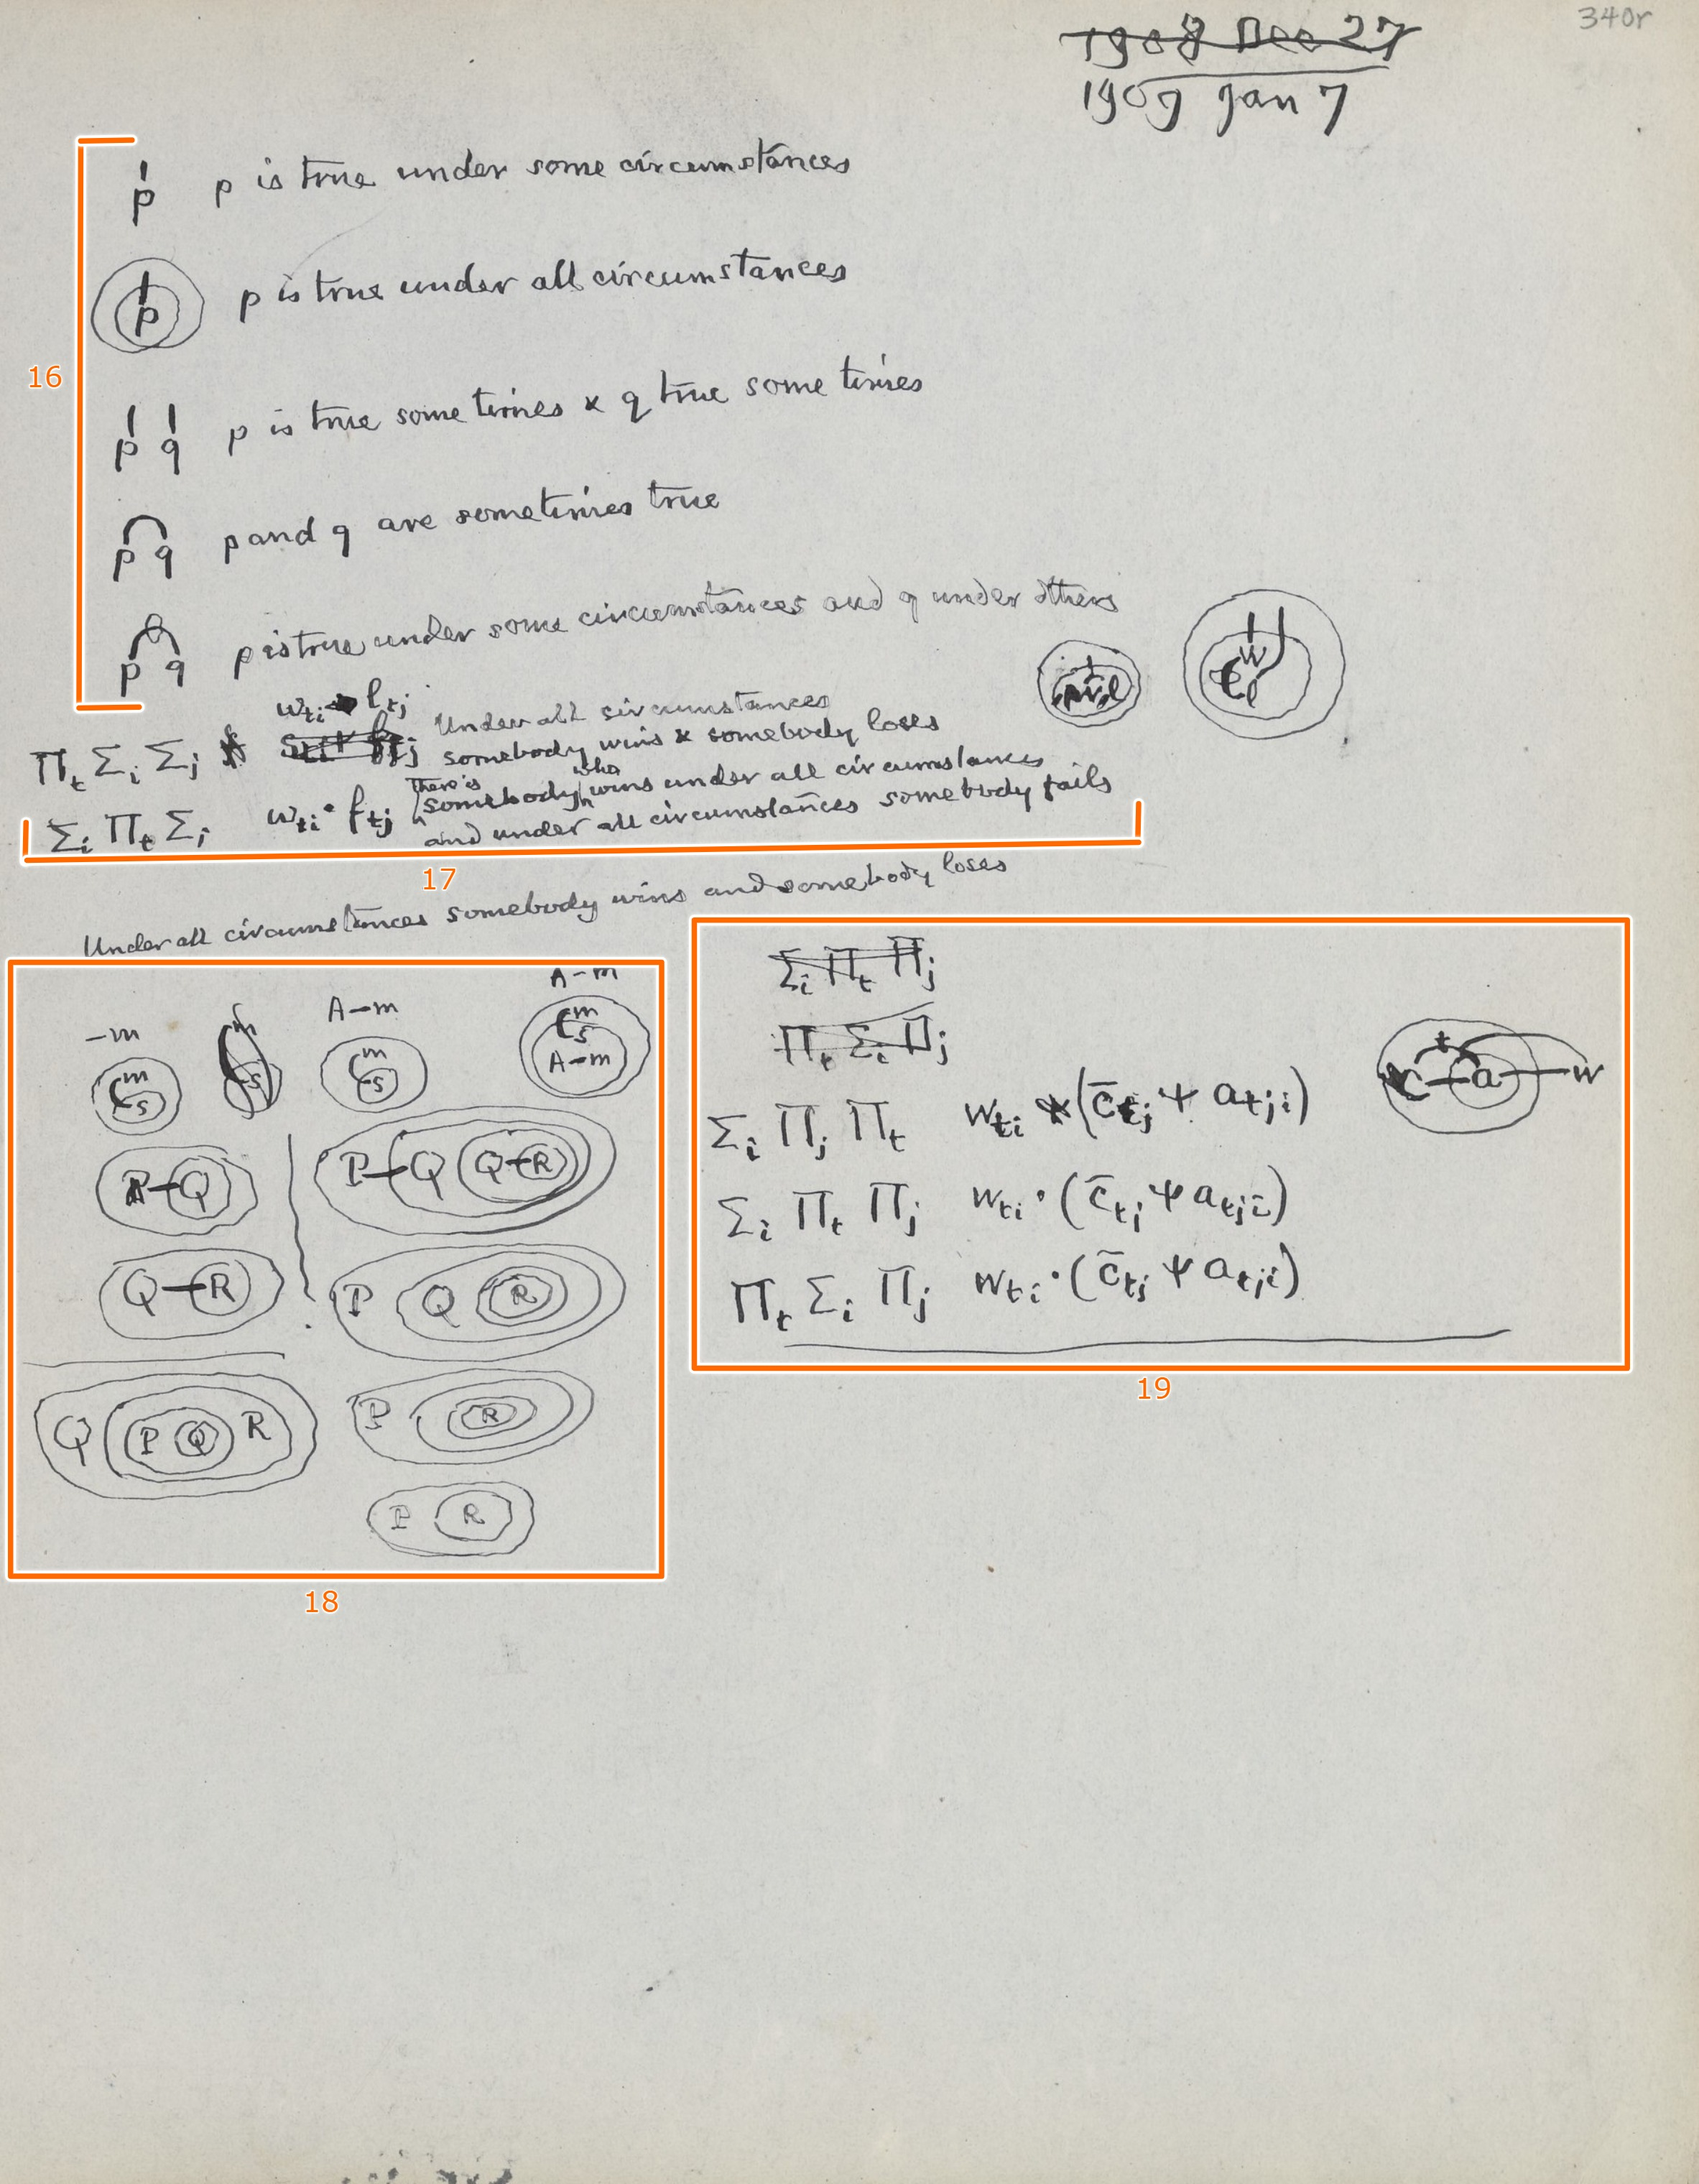
\includegraphics[width=\textwidth]{C:/Users/Brent/OneDrive/Documents/my LaTex project/Triadic logic/images/seq637.jpeg}
seq. 637 R.
\end{center}

\begin{center}
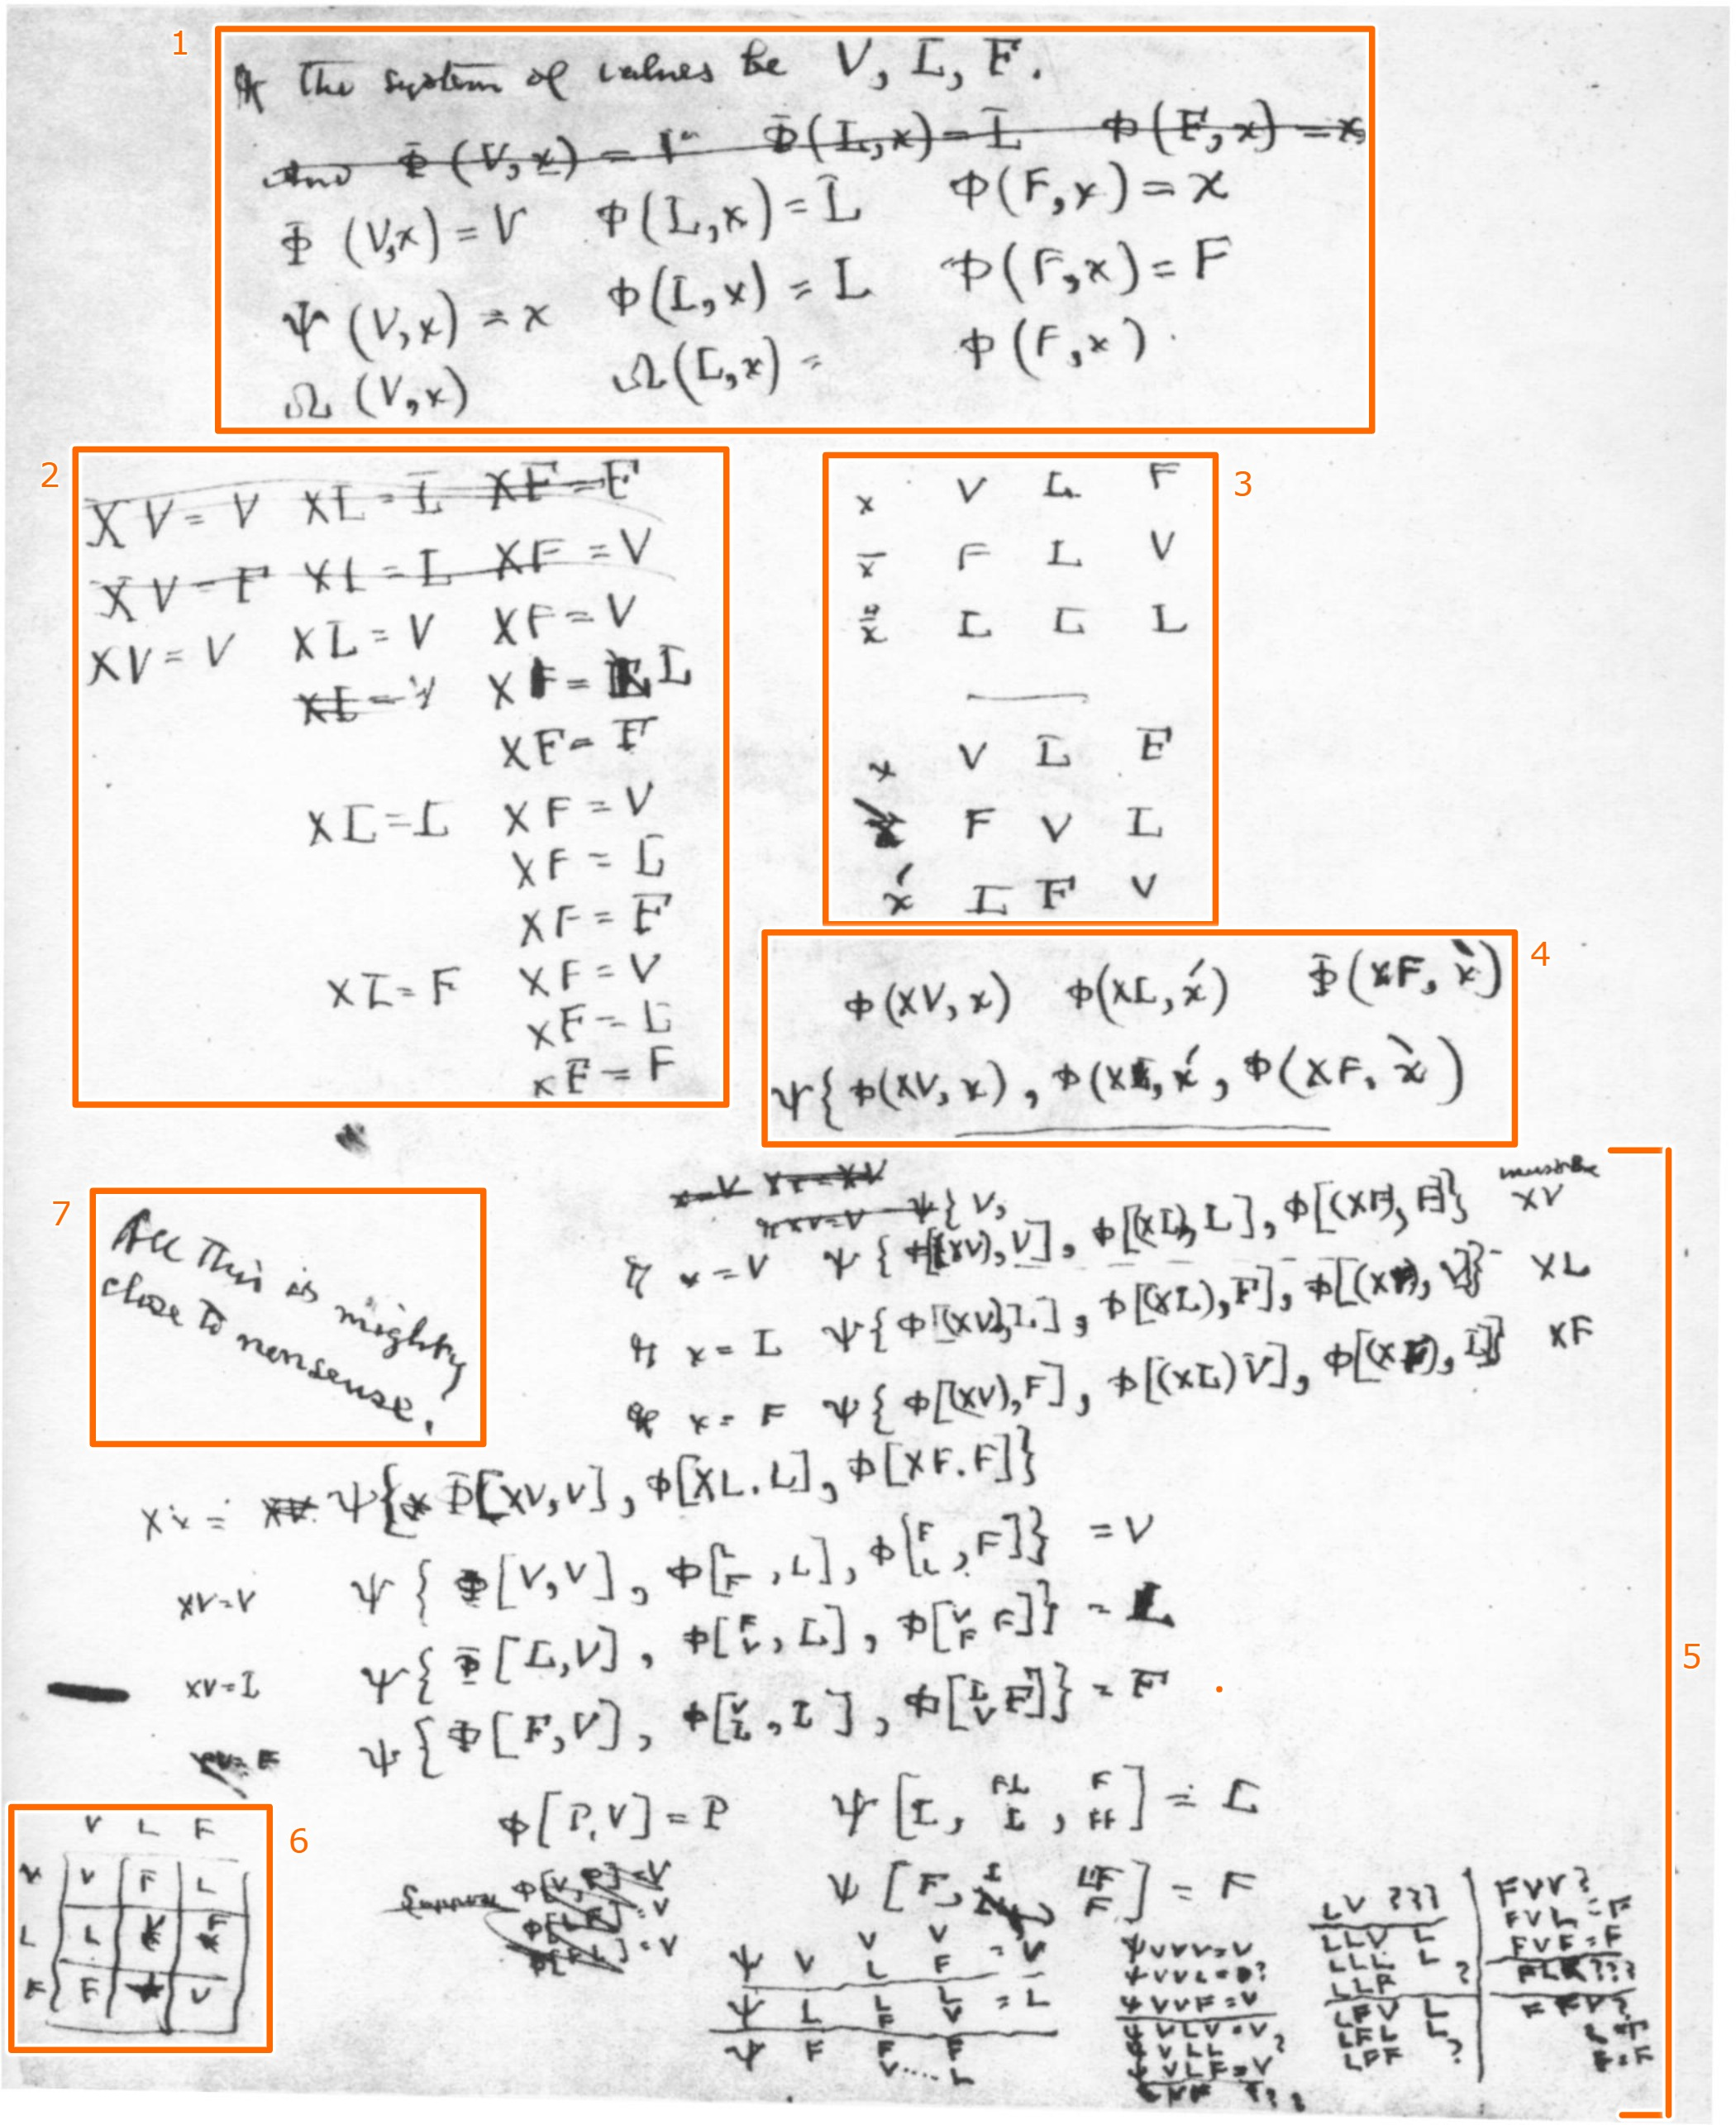
\includegraphics[width=\textwidth]{C:/Users/Brent/OneDrive/Documents/my LaTex project/Triadic logic/images/page one.jpeg}
First Page, seq. 638 V.
\end{center}

\begin{center}
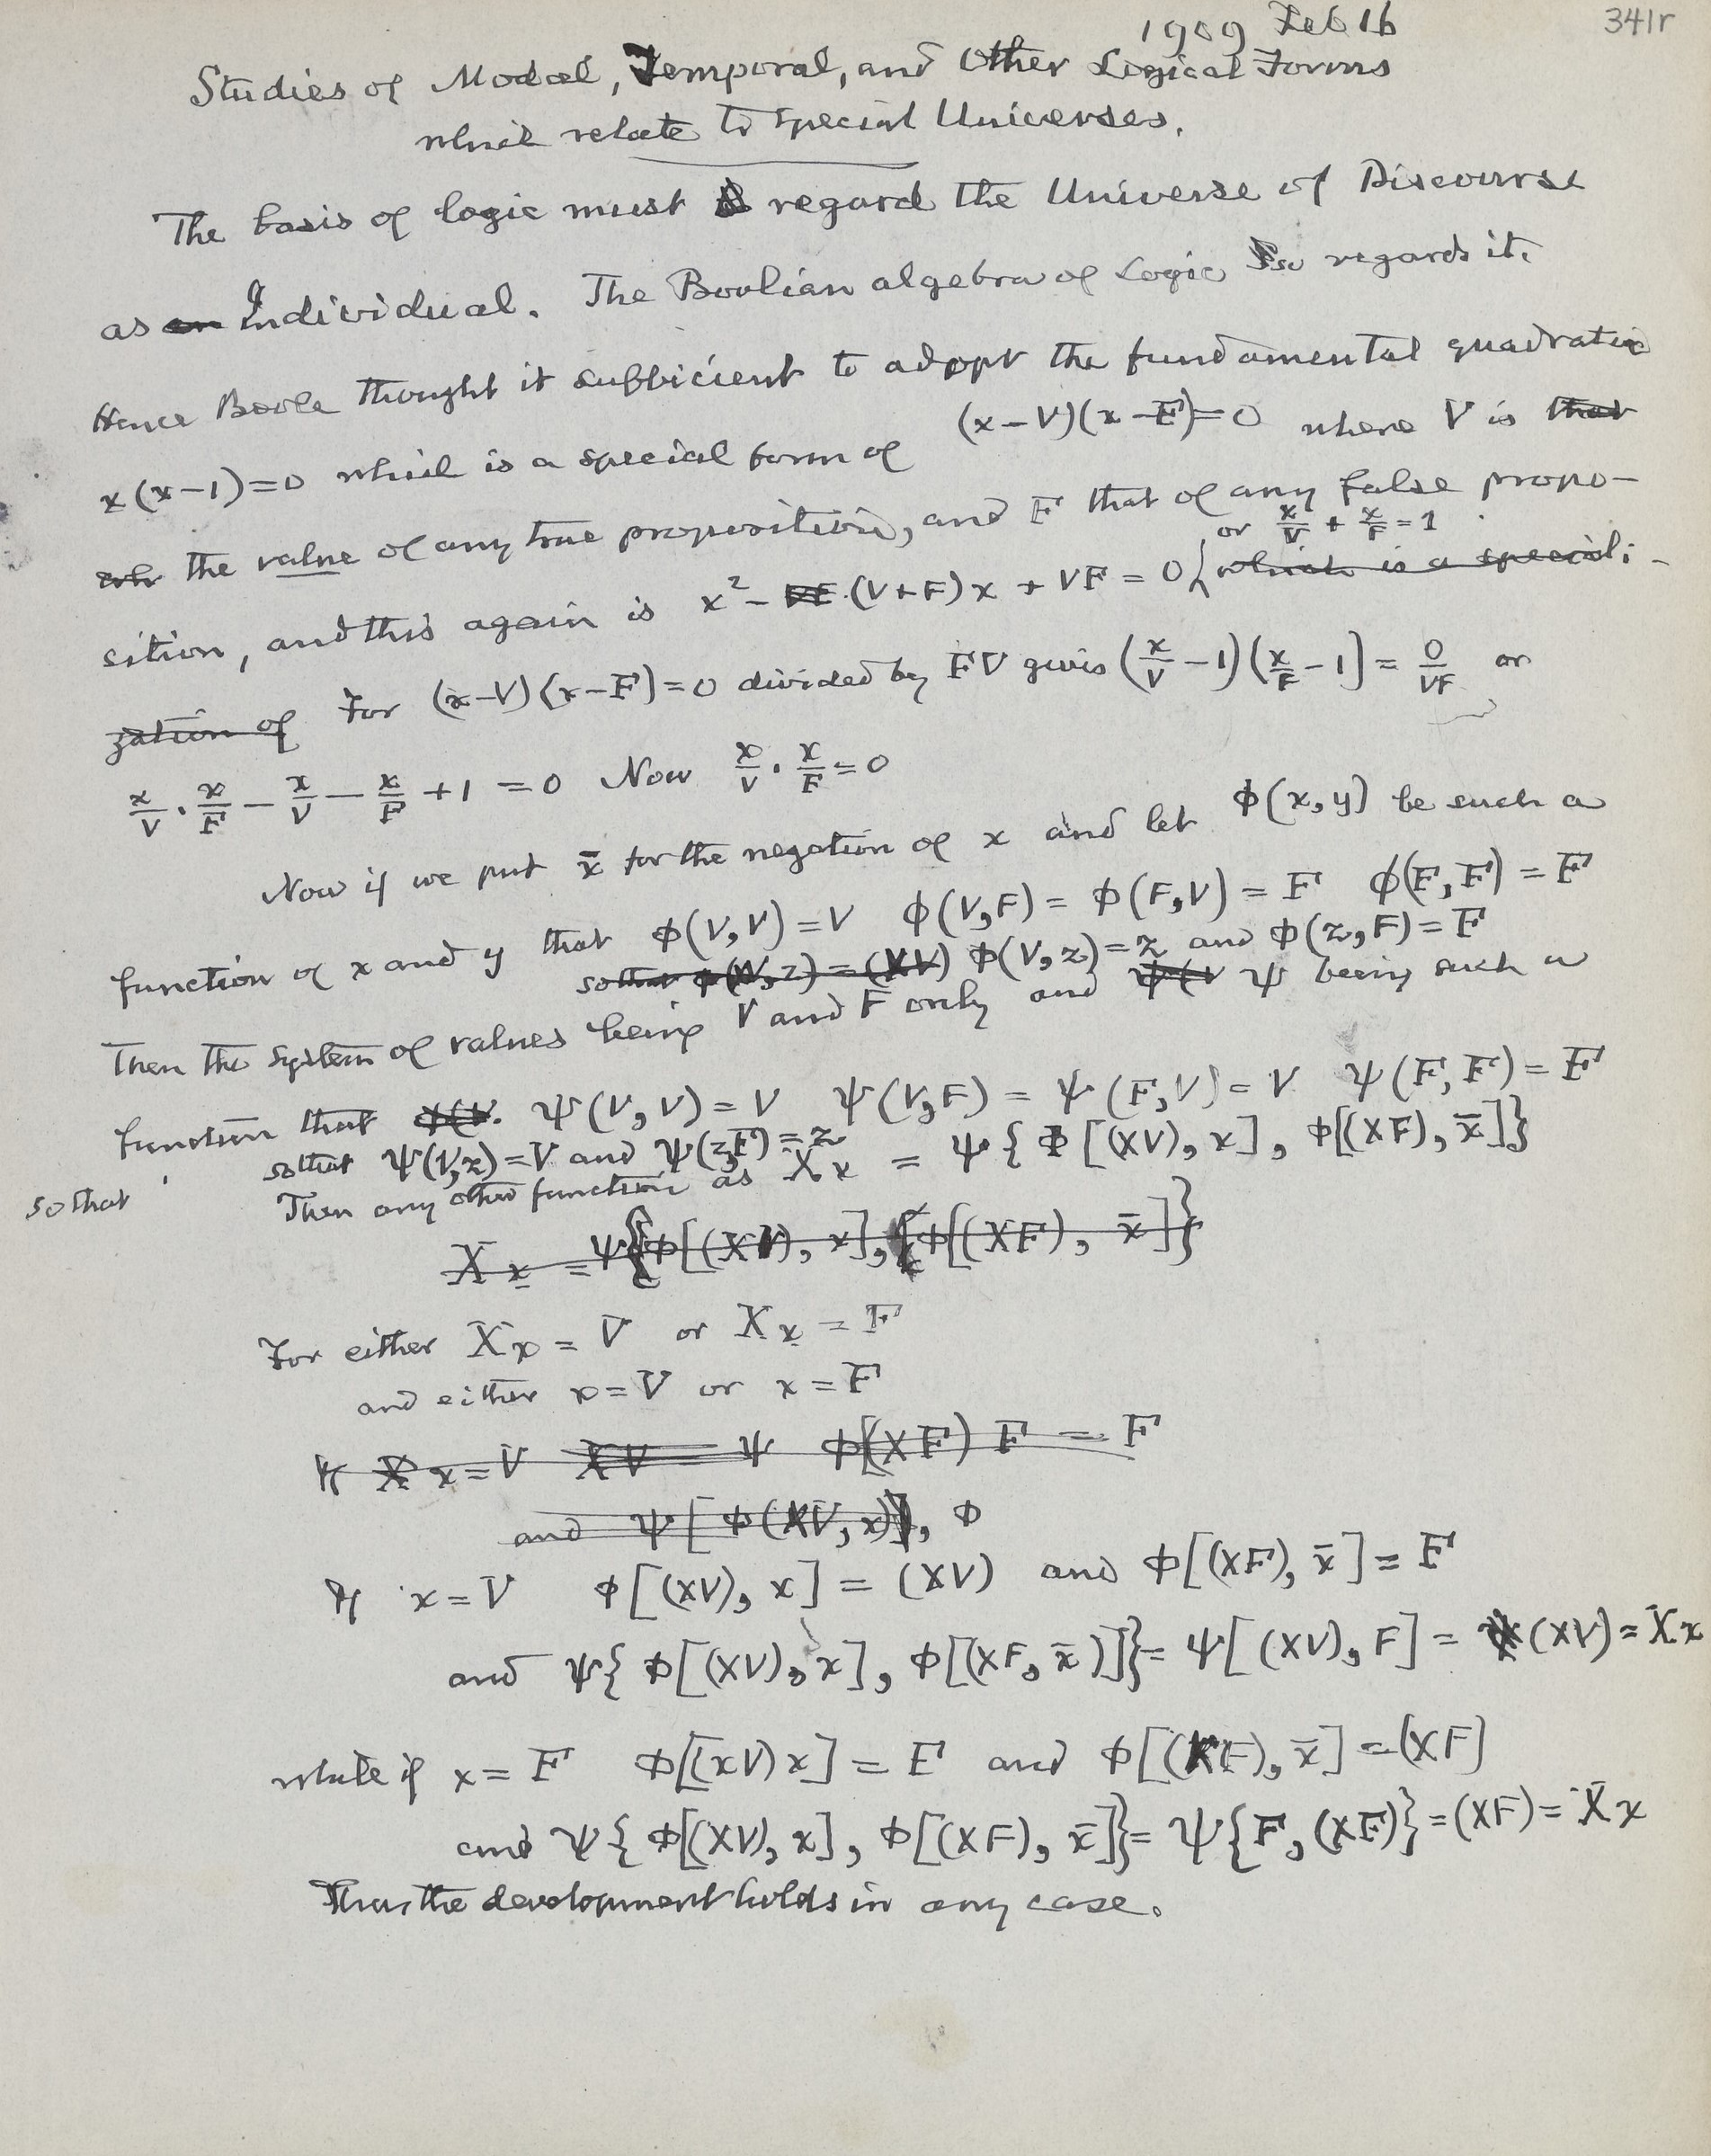
\includegraphics[width=\textwidth]{C:/Users/Brent/OneDrive/Documents/my LaTex project/Triadic logic/images/seq639.jpg}
seq. 639 R.
\end{center}

\begin{center}
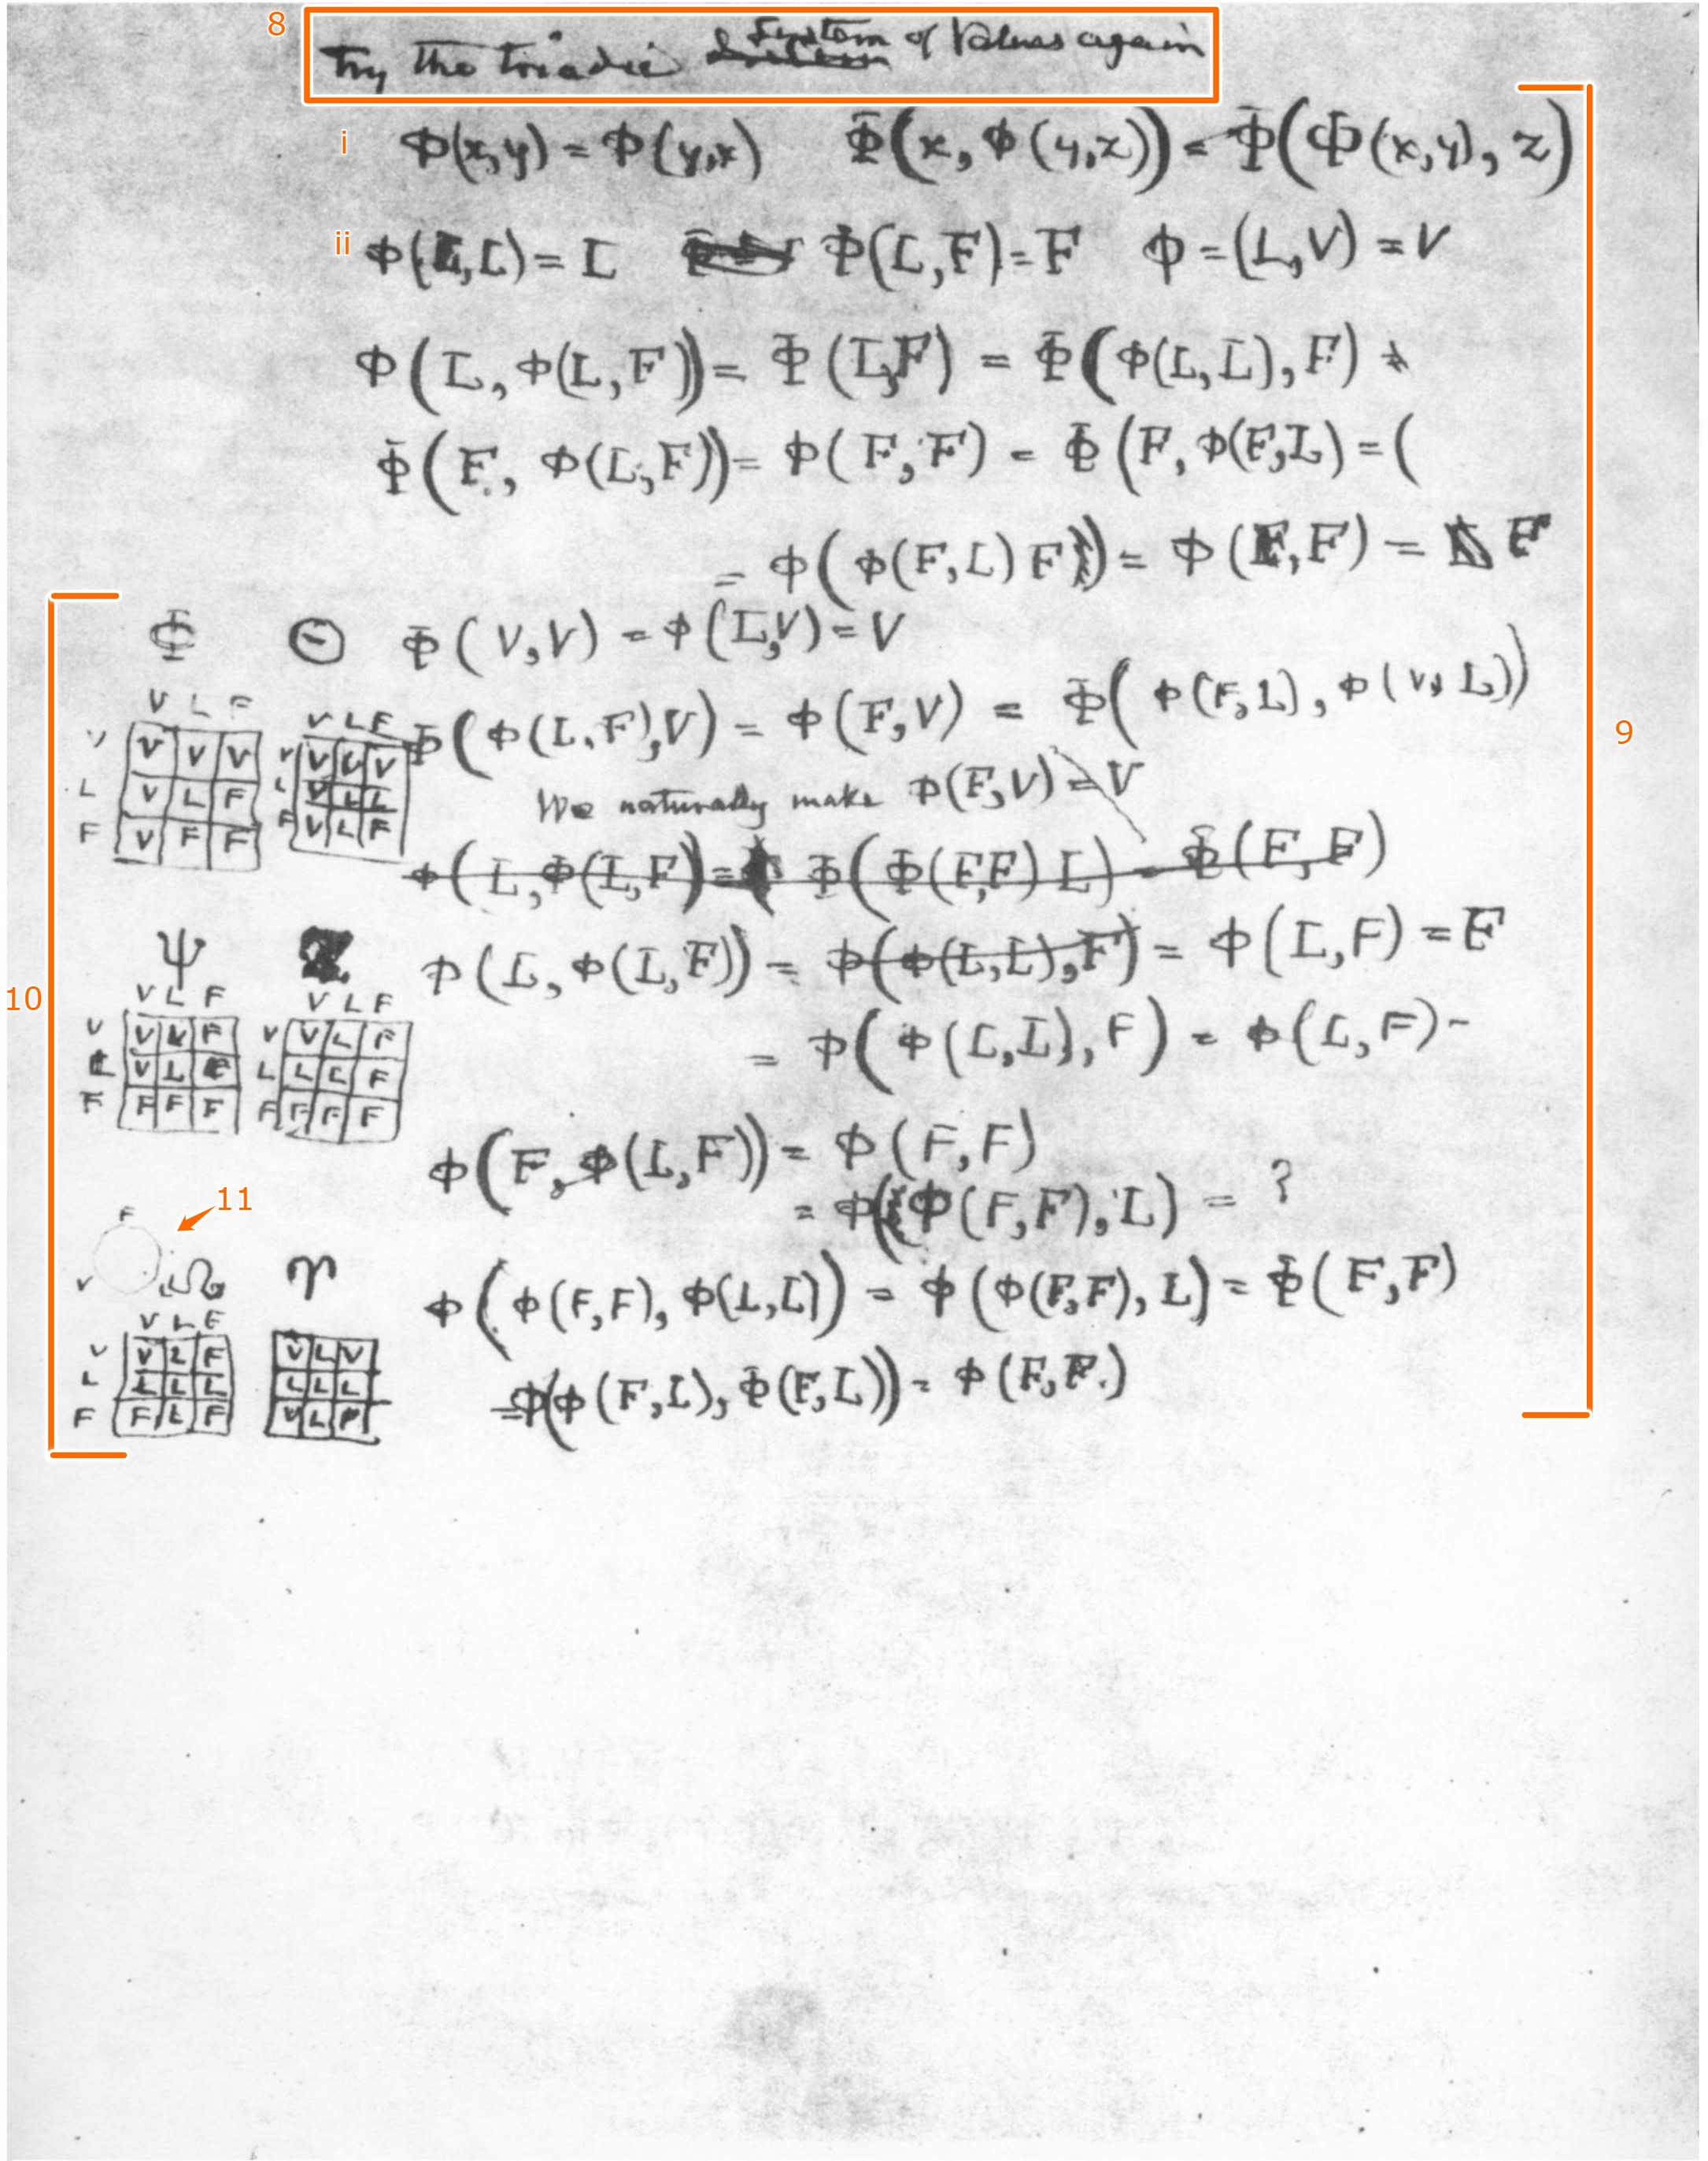
\includegraphics[width=\textwidth]{C:/Users/Brent/OneDrive/Documents/my LaTex project/Triadic logic/images/page two.jpeg}
Second Page, seq. 640 V.
\end{center}

\begin{center}
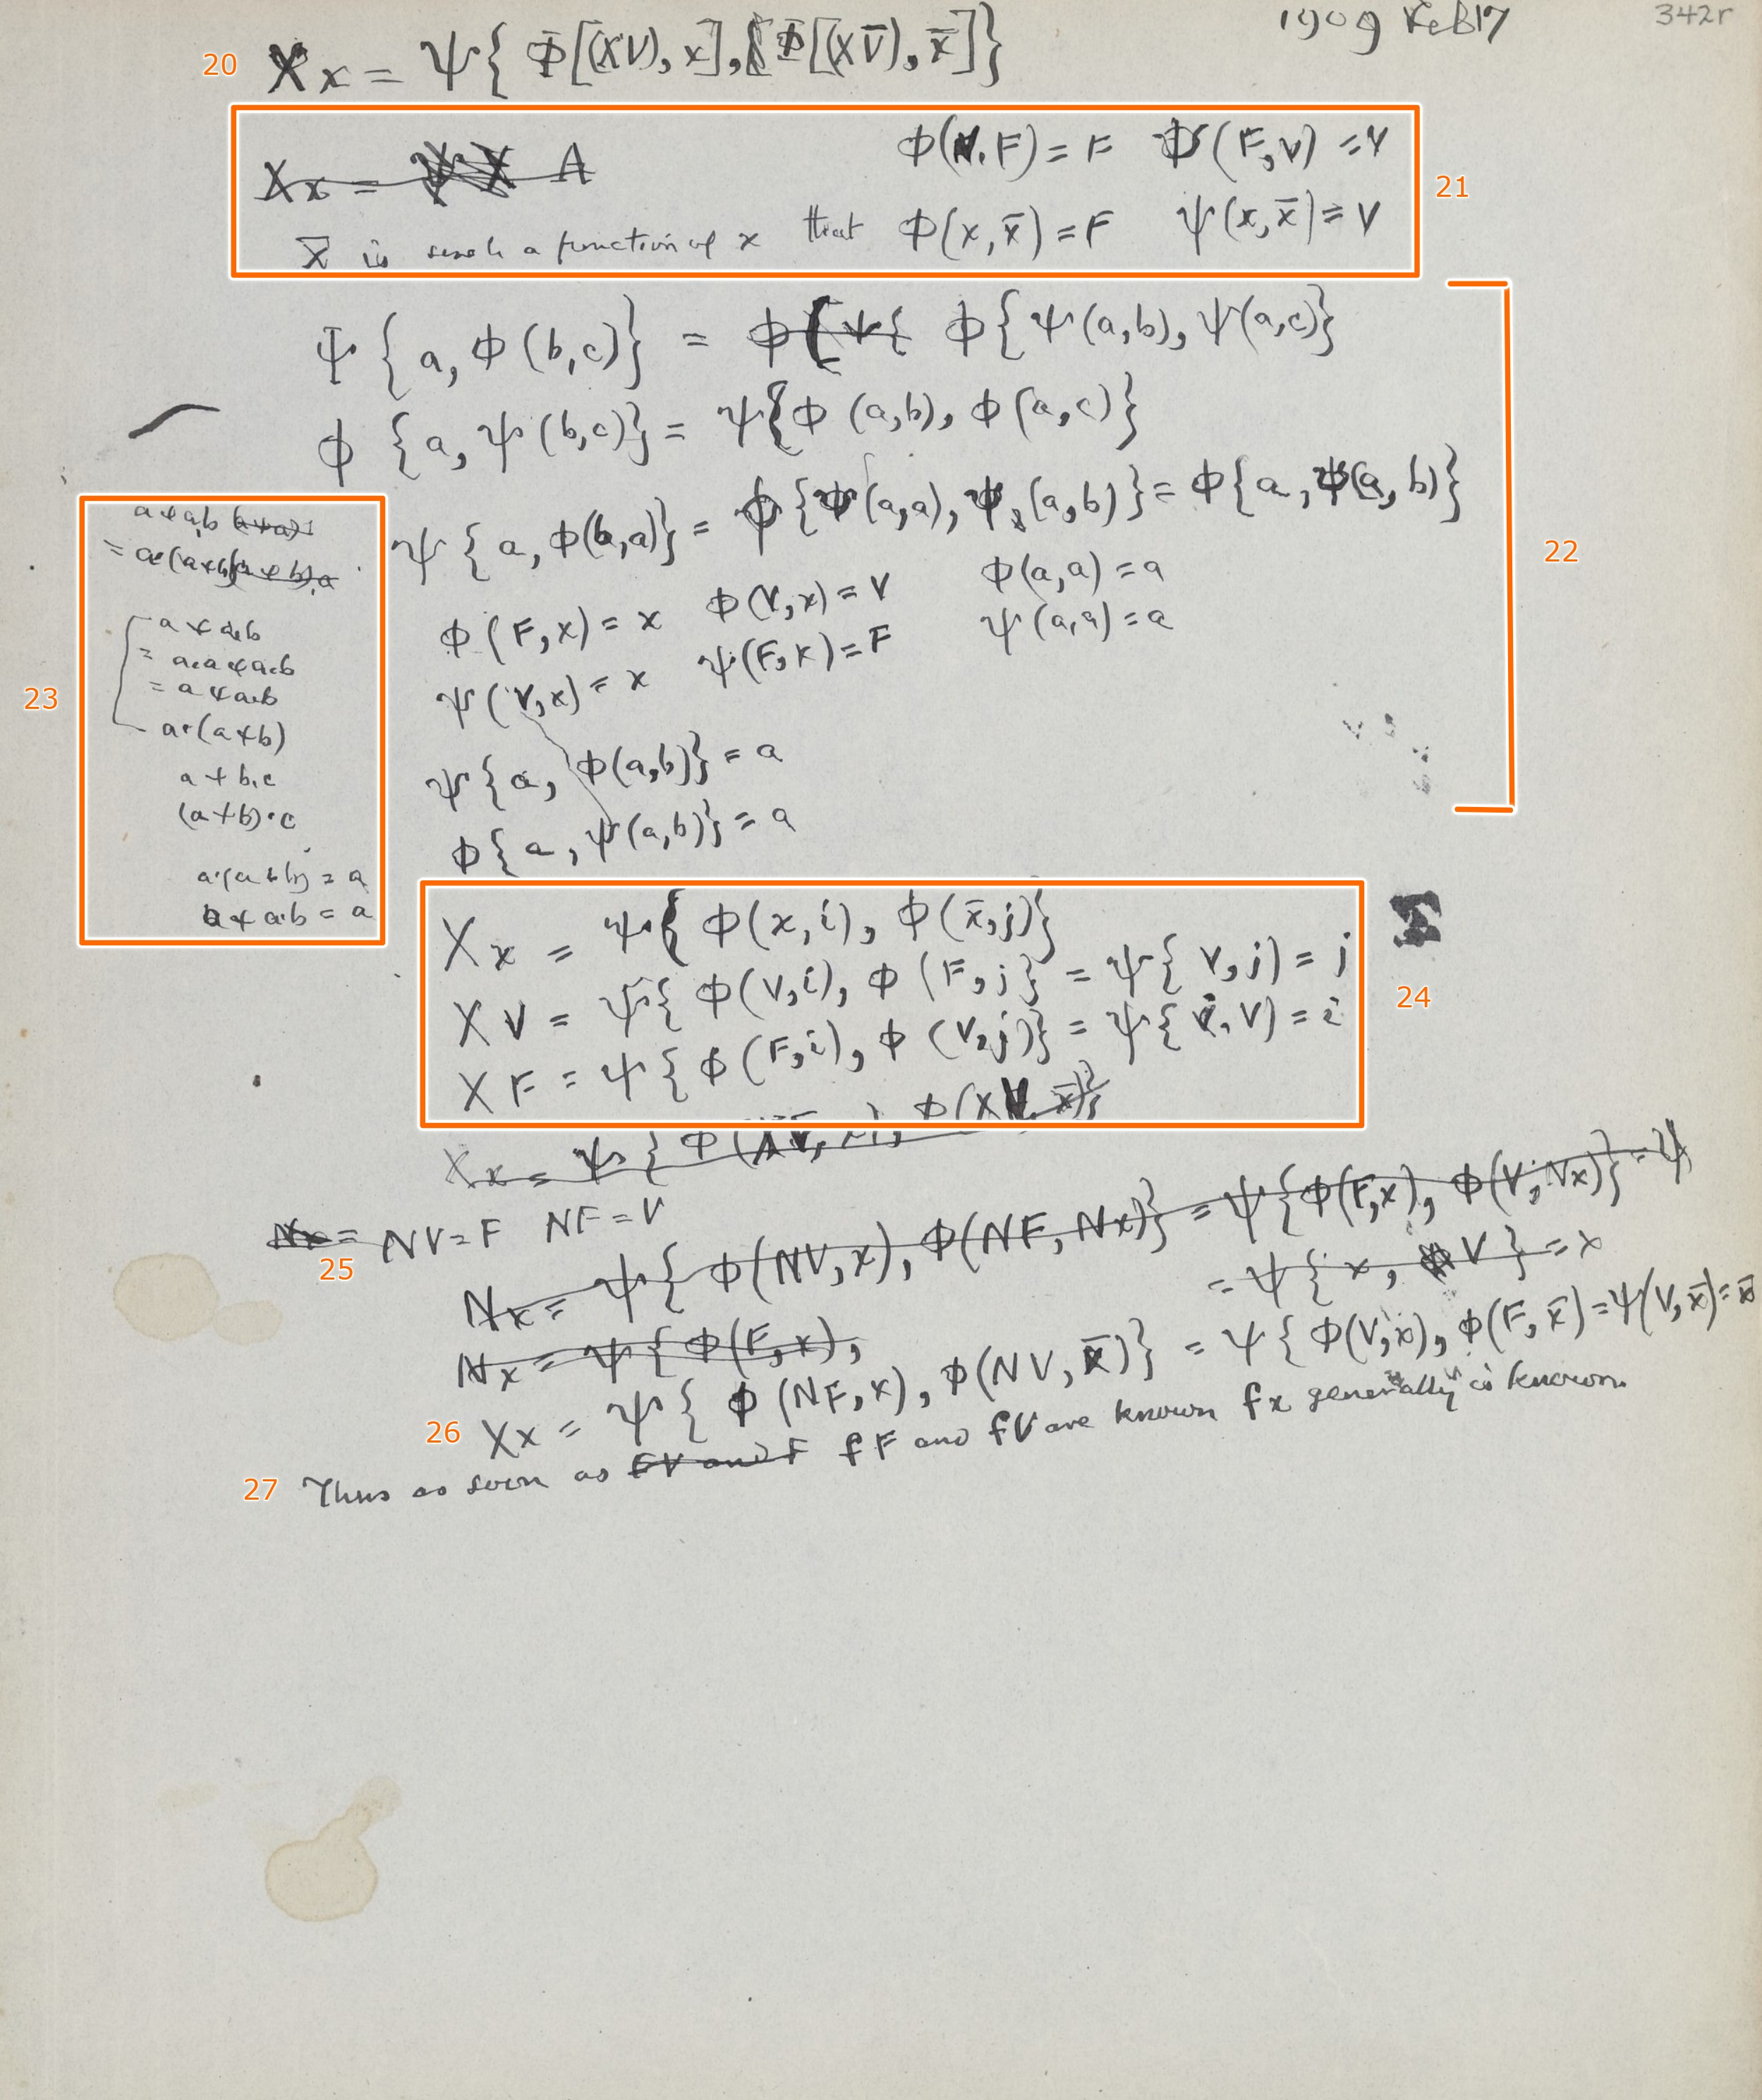
\includegraphics[width=\textwidth]{C:/Users/Brent/OneDrive/Documents/my LaTex project/Triadic logic/images/seq641.jpeg}
seq. 641 R.
\end{center}

\begin{center}
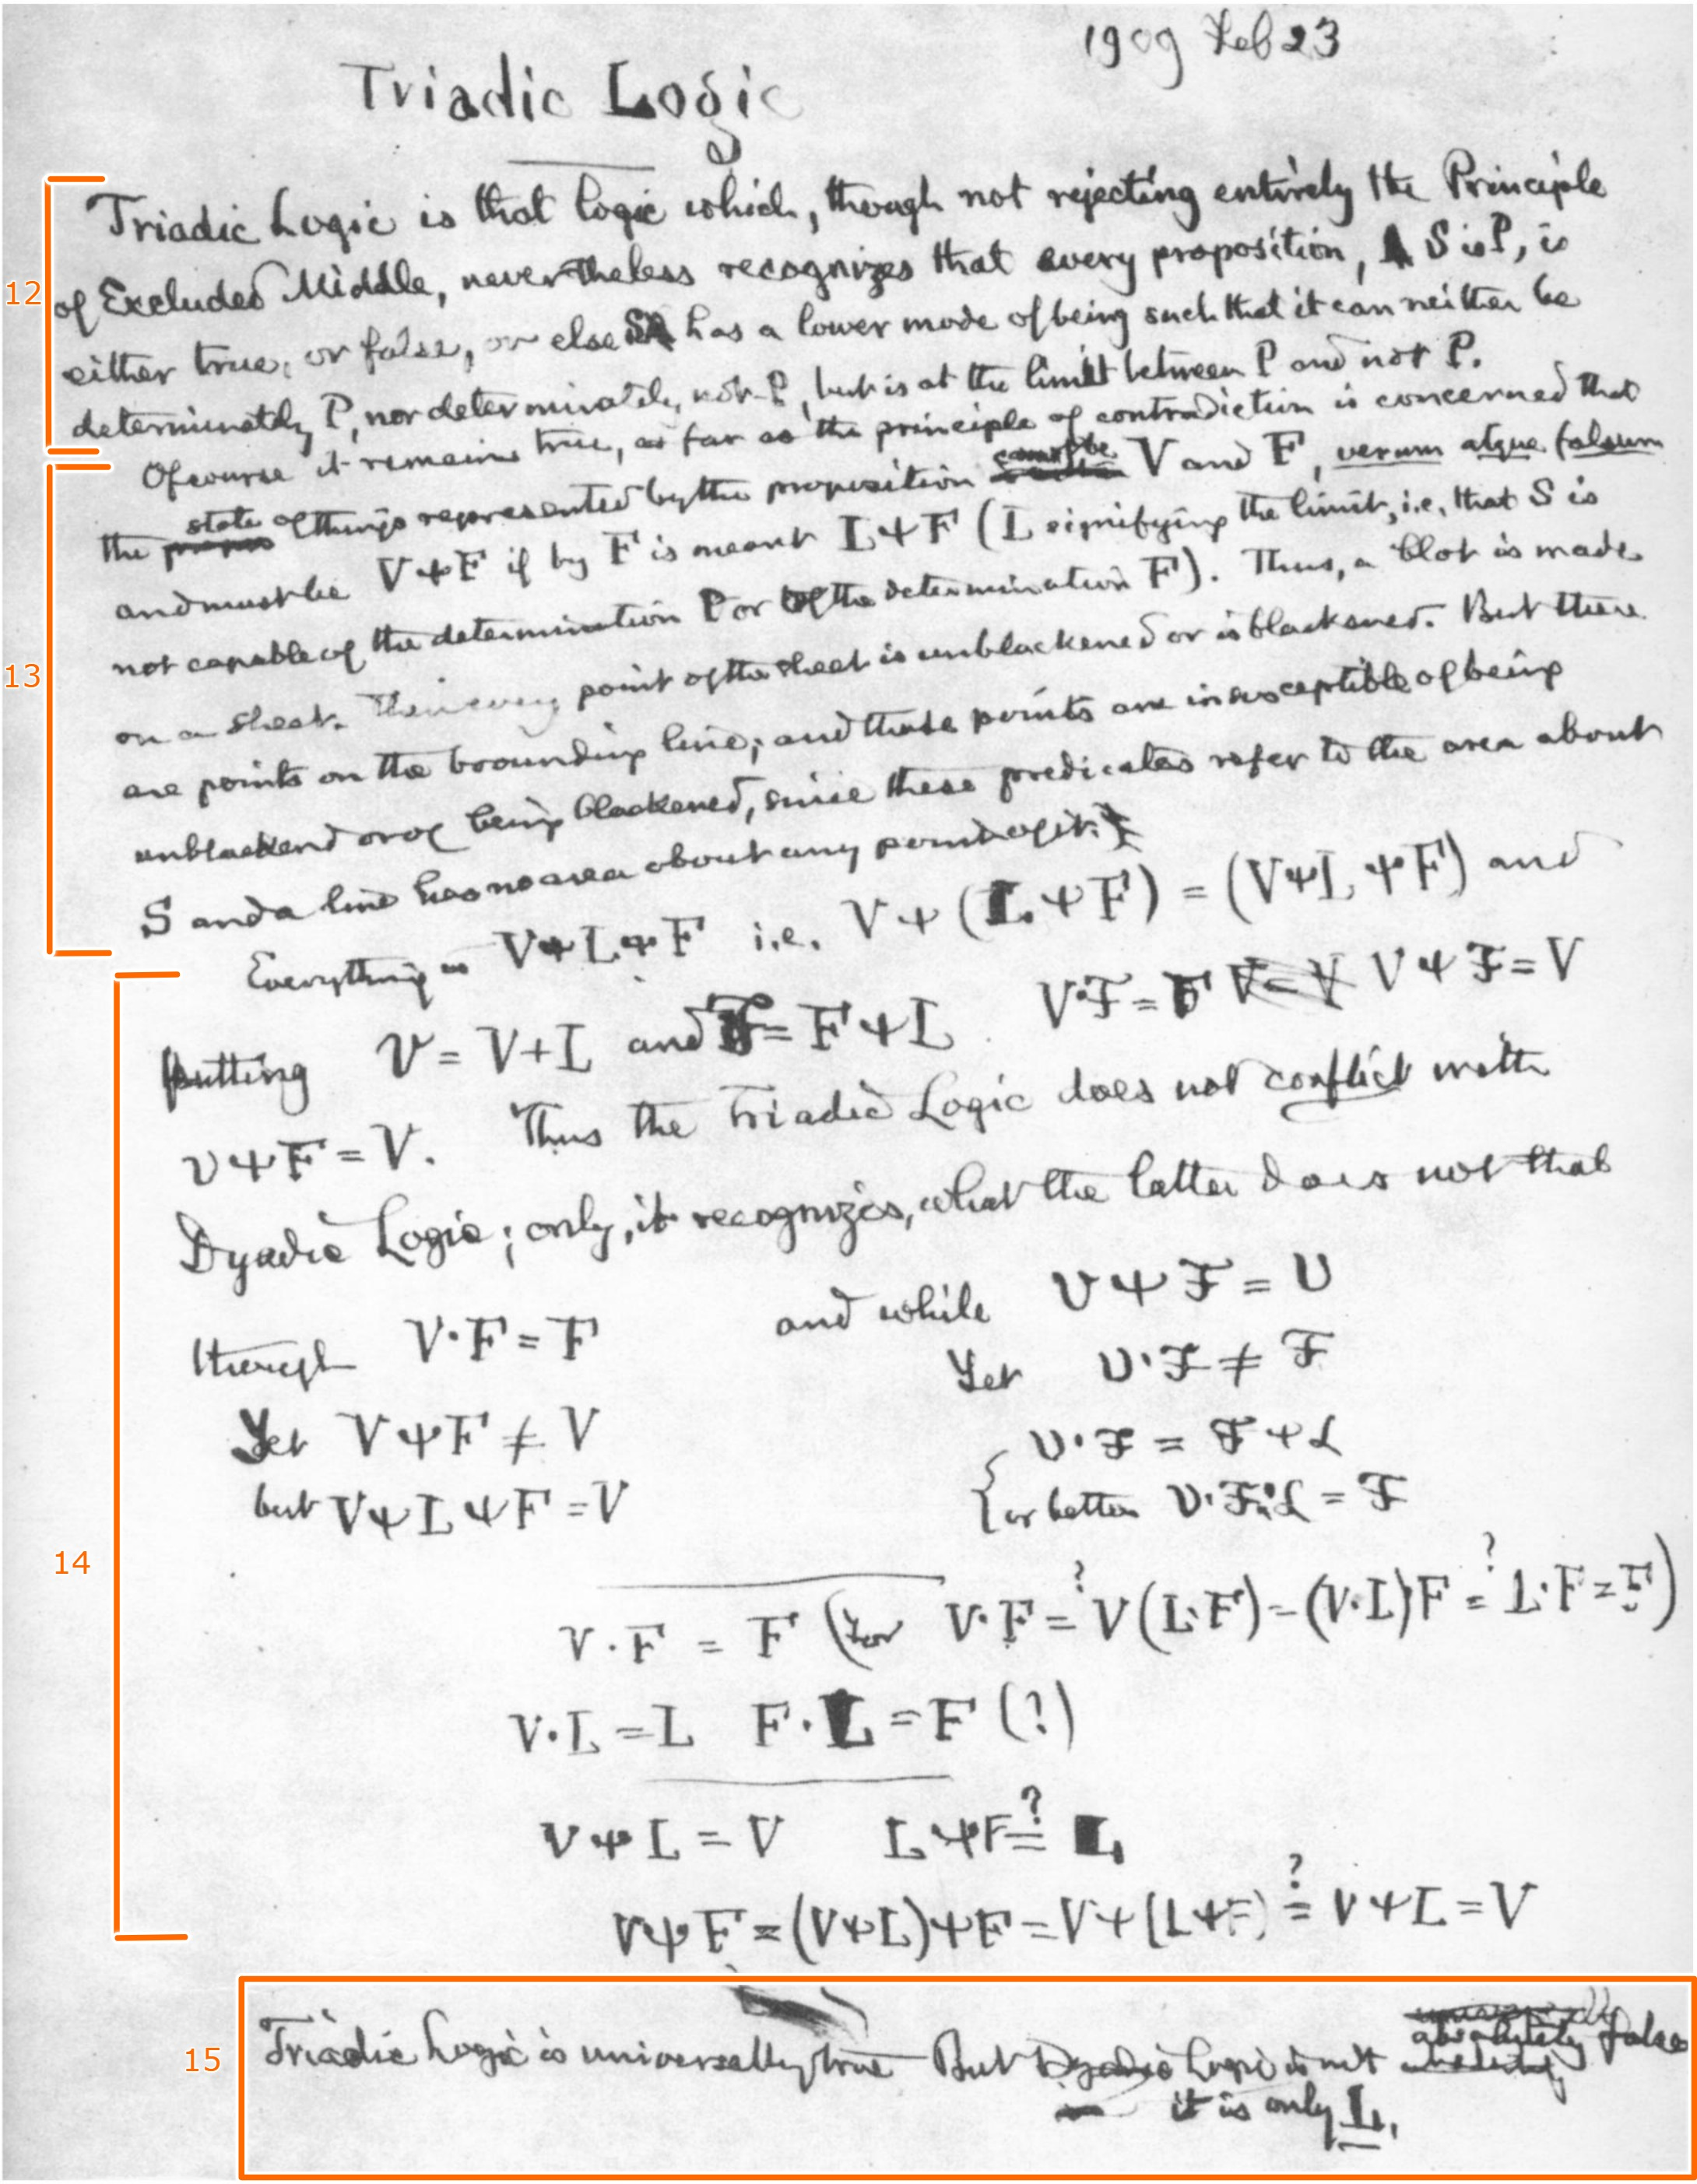
\includegraphics[width=\textwidth]{C:/Users/Brent/OneDrive/Documents/my LaTex project/Triadic logic/images/page three.jpeg}
Third Page, seq. 645 R.
\end{center}

\bibliographystyle{chicago}
\bibliography{Triadbib}

\end{document}
